En el capítulo anterior se ha realizado una introducción y un repaso a los conceptos
de  Web Semántica, \opendata, \linkeddata y \lod, en los cuales se ha podido comprobar
la diversidad de iniciativas, enfoques y estrategias que se están desarrollando de distintos ámbitos 
con el objetivo de hacer realidad la \wod. En el contexto
de las licitaciones públicas la aplicación de estos principios resulta clave para impulsar
la competitividad y la transparencia en los procesos administrativos que forman parte
de la contratación pública, no obstante una de las carencias que se puede vislumbrar
es la falta de estructuración de los procesos, métodos y tareas a definir
y desarrollar, para llevar a cabo una correcta realización práctica de estos conceptos
cumpliendo de esta forma con los principios que se propugnan. Es por ello que a lo largo 
capítulo se realiza una clasificación de los procesos, métodos y tareas
a efectuar, así como una definición teórica de los mismos. De esta manera,
una vez que se contextualicen los métodos definidos en el ámbito de la contratación pública, se podrá verificar su eficiencia respecto
a otros enfoques, en algunos casos, demasiado abiertos, que se alejan de la resolución del proceso 
encaminado a la apertura de datos enlazados complicando la iniciativa, provocando una sensación
de inquietud y duda, tanto por parte de los encargados de liberar los datos como 
por los que deben consumirlos.

Una primera clasificación de estos métodos, realizada recientemente~\cite{cold}, los enclava en dos grandes grupos:
\begin{enumerate}
 \item Publicación. Orientados a seleccionar los datos a liberar y a llevar a cabo
todas las actividades relacionadas con los mismos: modelado, diseño de URIs, formatos
de salida, etc.
 \item Consumo. Orientados a establecer los mecanismos de reutilización de datos enlazados
en distintas aplicaciones o bien en otros \datasets. Entre las actividades que lleva aparejadas
este gran grupo estaría: la consulta, enriquecimiento, calidad, establecimiento de cachés, etc.
\end{enumerate}

Sin embargo, estos dos grandes grupos pueden ser divididos en distintos tipos de métodos, que si bien
pueden encajar en distintos momentos de la generación de \linkeddata, la definición de los mismos debe ser única en cada caso. Existen
métodos y, en consecuencia, actividades que se han de reutilizar en distintos procesos con diferente denominación, de esta manera 
los métodos relacionados con la producción de datos enlazados estarán en estrecha relación
con aquellos que se encarguen de actualizar o consolidar los datos, por ejemplo un método que lleve
a cabo la tarea de descubrimiento automático de \datasets será de gran utilidad tanto en producción como en consumo o actualización. 
Por todo ello, además de proveer una clasificación de métodos semánticos, ver Figura~\ref{fig:metodos-clasificacion}, y distintas actividades 
relacionadas, se deben alinear con los ciclos de vida que se repasan en la Sección~\ref{gld}.


\begin{figure}[!htb]
\centering
	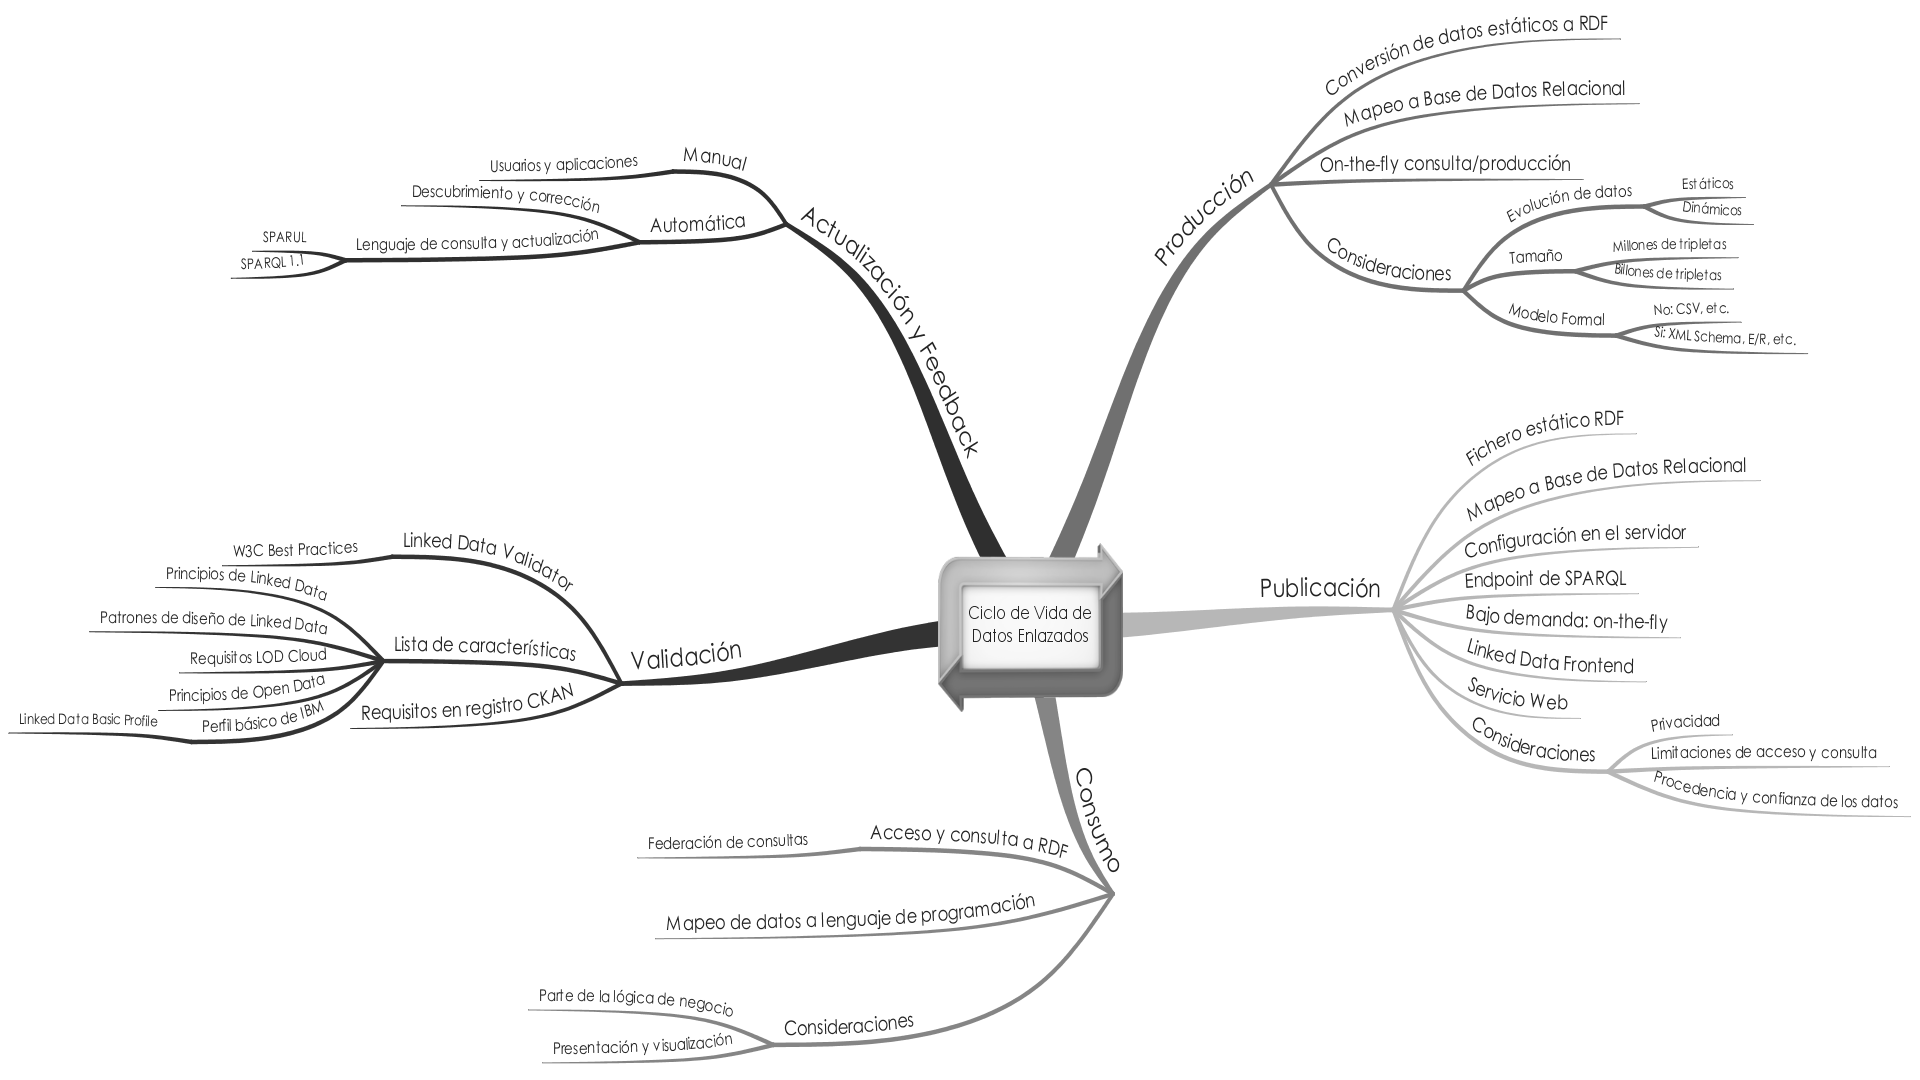
\includegraphics[width=16cm]{images/phd/ldl}
\caption{\textit{Clasificación de Métodos Semánticos}.}
\label{fig:metodos-clasificacion}
\end{figure}

Para llevar a cabo una nueva definición se necesita precisar qué procesos se deben contemplar en la apertura y enlazado
de datos, una vez definidos se identifican los métodos que se pueden aplicar y dentro de los mismos las tareas a ejecutar. 
Por ejemplo, en el proceso de ``Producción'' se deberá identificar los datos a transformar, seleccionar un esquema de URIs y validar la transformación. 
Por lo tanto, tenemos una descripción de 3 niveles: proceso, método semántico y tarea, que intentan dar respuesta a las siguientes preguntas, ver Tabla~\ref{tabla:procesos}. La selección
de estos procesos, métodos y tareas se ha llevado a cabo tratando de factorizar las actividades presentes en los distintos ciclos de vida de los datos enlazados.

\begin{figure}[!htb]
\centering
	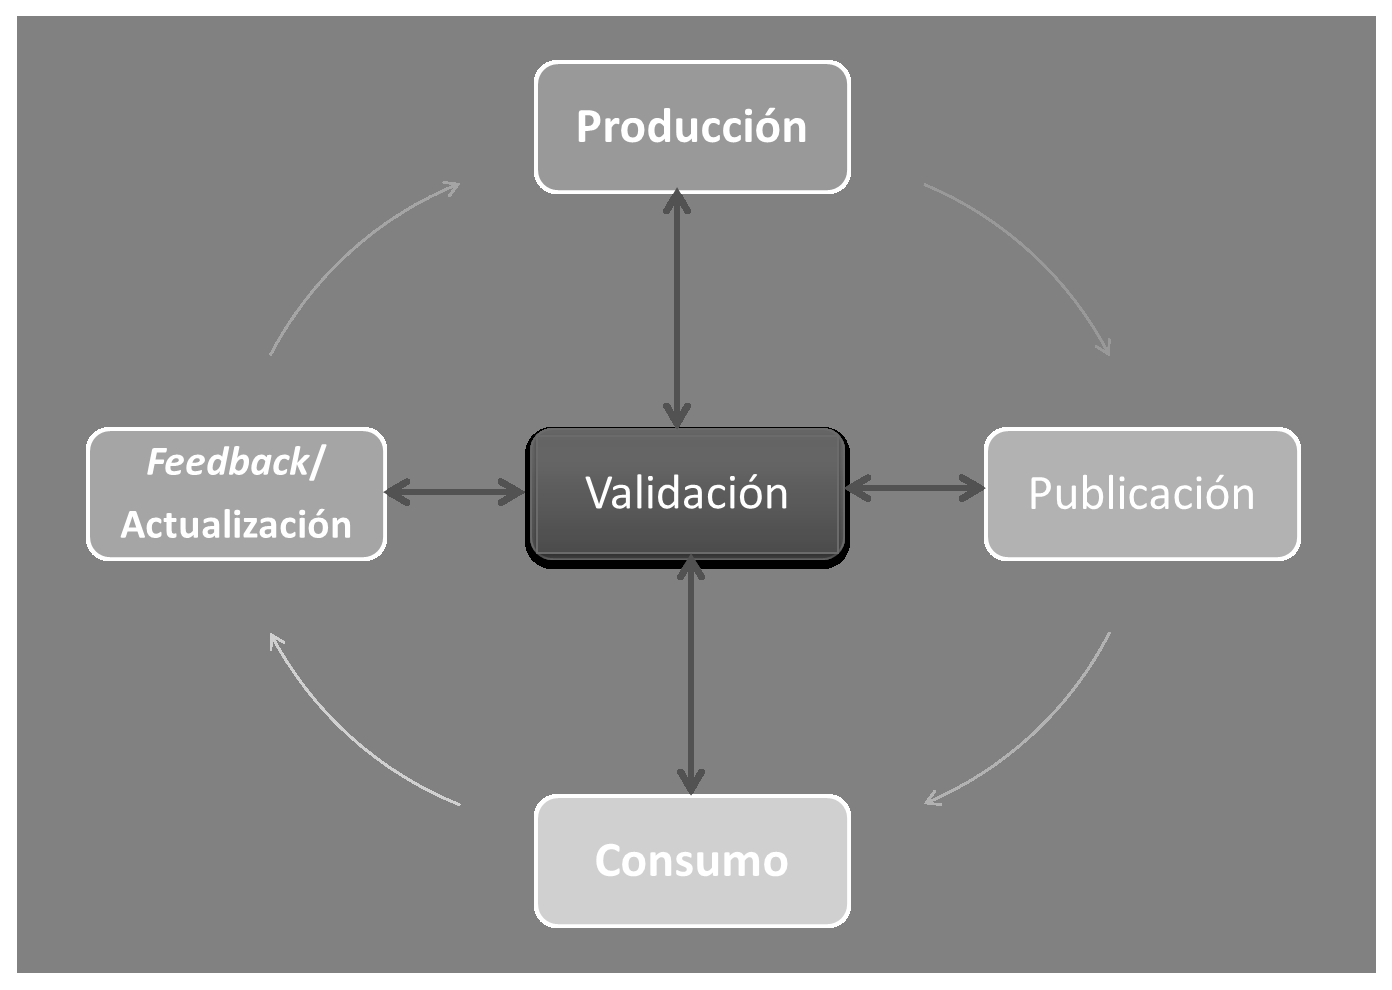
\includegraphics[width=14cm]{images/phd/lld}
\caption{Procesos en \linkeddata.}
\label{fig:metodos-clasificacion}
\end{figure}


\begin{longtable}[c]{|p{6cm}|p{8cm}|} 
\hline
  \textbf{Proceso} &  \textbf{Pregunta} \\\hline
\endhead
Producción & ¿Qué datos y cómo los transformo? \\ \hline
Publicación & ¿Cómo público los datos transformados? \\ \hline
Consumo & ¿Cómo reutilizo los datos enlazados disponibles? \\ \hline
Realimentación & ¿Cómo actualizo y mejoro mis datos enlazados? \\ \hline
Validación & ¿Cómo verifico que los datos enlazados en los distintos procesos son correctos? \\ \hline
\hline
\caption{Procesos y Preguntas en \linkeddata.}  \label{tabla:procesos}\\    
\end{longtable}



El proceso a seguir para desarrollar este capítulo es el siguiente:
\begin{enumerate}
 \item Definir los métodos semánticos de forma general en el marco de un proceso.
 \item Explicar los distintos enfoques que dan respuesta a ese método.
 \item Comentar las tareas que implica llevar a cabo el enfoque anterior.
 \item Ejemplificar el método con un ejemplo transversal.
\end{enumerate}

\subsection{Ejemplo transversal}
Para ejemplificar cada una de las definiciones realizadas a lo largo de este capítulo se utilizará
un ejemplo de un conjunto de datos real. Se ha seleccionado la información disponible en el Nomenclátor
de Asturias 2010 realizado por la Sociedad Asturiana de Estudios Económicos e Industriales, ya que contiene
información de distintos ámbitos (nombres, estadísticas, etc.) e idiomas y facilita la comprensión y lectura del documento. 

\section{Definiciones Previas}
Durante este capítulo se utilizarán algunas de las definiciones ya realizadas
en las distintas especificaciones~\cite{RDF,citeulike:1556975,RDFS,owl2-primer,SparqlSemantics,Perez:2009:SCS:1567274.1567278} sobre el uso de Web Semántica y algunos
de los conceptos clave pertenecientes a la iniciativa de \linkeddata. 

\begin{description}

 \item [Tupla.] Siguiendo las definiciones utilizadas en el modelo relacional y en matemáticas. Una tupla
es una función que \textit{mapea} nombres con valores. En general, se trata de un conjunto de valores
$a_1,a_2...a_n$ que guardan una relación de orden entre sí, pueden contener valores repetidos y otros objetos dentro de sí.

\item [\textit{Dataset}.] Se puede definir como un conjunto de tuplas. Si se tiene en cuenta que en la mayoría de los
casos al producir \linkeddata los datos se obtienen de una base de datos relacional, \gls{XML}, texto separado por comas, etc., cada uno de los almacenes especifican una forma de guardar tuplas para generar un \dataset.

\item [\textit{Internationalized Resource Identifiers} (\gls{IRI}s).] Habitualmente se utiliza la denominación de IRI (\gls{RFC}-3987) para referirse
a una generalización de las \gls{URI}s y URLs (RFC-3986), siendo totalmente compatibles con las definiciones de las anteriores. 
Normalmente se presentan de la siguiente forma $<IRI>$ y pueden ser relativas respecto a un IRI base o completas.

En las definiciones formales de \gls{RDF} y \gls{SPARQL} se utiliza el término IRI pero por su definición puede ser utilizado
también el término URI. En el ámbito de \linkeddata se puede afinar aún más y utilizar la siguiente nomenclatura:
 $IRI \longrightarrow  URI \longrightarrow  HTTP$ $URI$

\item [\textit{Uniform Resource Identifier}.] El concepto de URI surge como una cadena de caracteres para identificar de manera única
a un elemento, en el contexto de la Web Semántica se ha utilizado este término para identificar recursos. Dentro
de la definición de URI encaja \textit{Uniform Resource Locator} (\gls{URL}), que además de proveer información de nombrado sobre el elemento
especifica cómo se ha de acceder a él. En el documento~\cite{RDF} se hace referencia al término HTTP URIs para identificar
a aquellas URIs que utilizan el esquema de nombrado \gls{HTTP} para identificar a los recursos dentro de la iniciativa de la Web Semántica.

\item [Modelo RDF.] Aunque ya se ha comentado en la Sección~\ref{semantica} el modelo RDF, cabe recordar su definición, RDF
sigue y cumple con los principios y características de interoperabilidad, extensibilidad, capacidad de evolución
y descentralización elaborados por el \gls{W3C}. En particular, el modelo RDF se diseñó para tener un modelo de datos
simple con una semántica formal y capacidades de inferencia basado en un vocabulario que hace uso de URIs para nombrar
a los elementos. En el universo RDF, los elementos a modelar son un conjunto de recursos, en esencia todo
aquello que sea susceptible de tener un URI. El lenguaje utilizado para describir estos recursos se compone
de un conjunto de predicados (binarios). Las descripciones de recursos en RDF se basan en la estructura
$<s,p,o>$ (sujeto, predicado, objeto), en los cuales los predicados y los objetos son también recursos o 
literales (en el caso de los objetos). Por otra parte, sujetos y objetos pueden ser anónimos, así tienen URI
pero sólo de forma local, formando lo que se denominan \textit{blank nodes} cuyo uso se ha evaluado y juzgado~\cite{DBLP:conf/semweb/MalleaAHP11} 
recientemente.

En conclusión el modelo RDF consta de unos principios para construir un vocabulario 
bajo una determinada semántica, en muchos casos RDFS~\cite{RDFS} u \gls{OWL}~\cite{owl2-primer}, permitiendo así la herencia
de clases y propiedades, definición de tipos y otras características. Este modelo
es especificado en una serie de documentos que cubren su semántica, sintaxis, serilización, etc.

\item [Tripleta RDF.] Es una tupla $(s,p,o) \in (I \cup B) \times I \times 
(I \cup L \cup B)$, en el cual $I$ es el universo de todos los posibles recursos que se pueden identificar
por un IRI, $B$ es un conjunto infinito de recursos no nombrados y $L$ es el conjunto
de todos los literales RDF.

\item [Grafo RDF.] Un conjunto de tripletas RDF se interpreta estructuralmente como un grafo
RDF $\mathcal{G} =(V,E)$, donde $V$ es el conjunto de vértices, $V \subseteq (I \cup B \cup L)$,
y $E$ es el conjunto de ejes, $E \subseteq V \times I \times 
V$. Para cada tripleta $(s,p,o)$ del modelo RDF existe
una arista dirigida, etiquetada con el predicado $p$, entre los vértices que representan el sujeto $s$ y el objeto $o$. Si este
grafo no tiene nodos en blanco se denomina \textit{ground}.

\item [Recurso RDF.] Es un conjunto de sentencias o tripletas $(s,p,o)$ RDF en las cuales el sujeto $s$ 
es constante, tiene la misma IRI.

\item [Grafo RDF nombrado.] Es un grafo RDF identificado por un IRI. 

\item [\textit{Dataset} RDF.] En la especificación de SPARQL~\cite{Sparql} y su semántica~\cite{SparqlSemantics} se habla
de \dataset RDF y se define como un conjunto $\mathcal{D} = \{\mathcal{G}, (<I_1>, \mathcal{G}_1), (<I_2>, \mathcal{G}_2)...(<I_n>,\mathcal{G}_n)\}$,
donde $\mathcal{G}$ y cada $\mathcal{G}_i$ son grafos RDF identificados a través de un IRI $I_i$ y $n\geq0$.
 Cada par $(<I_n>, \mathcal{G}_n)$ es un grafo nombrado en el cual $I_n$ es el identificador del grafo
$\mathcal{G}_n$; $\mathcal{G}$ es el grafo por omisión (\textit{default graph}) y contiene
todas las tripletas. 

Esta definición sobre un \textit{Dataset} RDF se puede extender para definir un modelo formal que sirva
para integrar información proveniente de distintas fuentes de datos dentro de un
repositorio RDF u otro sistema de almacenamiento. Un \dataset integra varios grafos RDF
$\mathcal{G}$, de forma que cada una de las tripletas se puede identificar, gestionar y referenciar
de forma separada. En el modelo de datos de RDF, utilizando grafos nombrados las sentencias forman parte del conjunto de datos o de un 
grafo nombrado $\mathcal{G}_n$ o bien del grafo por omisión $\mathcal{G}$.

Por lo tanto, un \dataset RDF puede representar información de distintos grafos RDF, si se añade
una nueva dimensión a la definición de tripleta RDF $(s,p,o,\mathcal{G})$ se obtienen 
``sentencias contextualizadas'', en las que los tres primeros elementos $(s,p,o)$ indican
una sentencia RDF y el cuarto elemento $\mathcal{G}$ representa el grafo en el que están
definidas. De esta forma un \textit{Dataset} RDF consta de un conjunto infinito de cuádruplas $(s,p,o,\mathcal{G})$. 
Esta definición es ampliamente utilizada en los repositorios RDF para identificar los distintos recursos y así
poder acceder mediante SPARQL a los recurso definidos en determinados grafos.


\item [Ontología.] Se define una ontología $\mathcal{O}$ como una tupla $\mathcal{C}$, $\mathcal{R}$, $\mathcal{I}$, $\mathcal{A}$, donde $\mathcal{C}$ es un conjunto de conceptos,  $\mathcal{R}$ es un conjunto de relaciones, $\mathcal{I}$ es un 
conjunto de instancias y  $\mathcal{A}$ es un conjunto de axiomas. Todos los conceptos, relaciones, instancias
y axiomas se expresan a través de un lenguaje como OWL o F-Logic que permite expresar un determinado formalismo lógico. 
Esta visión de una ontología encaja con la definición realizada en OKBC, los conceptos se corresponderían con clases en OKBC, relaciones con ``slots'', ``facets'' con tipos de axiomas y los ``individuals'' 
corresponderían con instancias.

La necesidad de definir el concepto de ontología reside en que las descripciones de recurso en RDF deberán
haber sido modeladas previamente de acuerdo a un modelo formal. Teniendo en cuenta que en el contexto objeto de estudio se utilizarán
ontologías, de este modo un recurso RDF se presenta como una instancia de un concepto de una ontología $\mathcal{O}$ que 
especifique el conocimiento de este dominio.

\item [\textit{Mapeo} entre instancias.] Los \textit{mapeos} entre conceptos e instancias de una ontología $\mathcal{O}$ y en consecuencia
de recursos RDF han sido ampliamente estudiados~\cite{NM00} en el campo de los servicios web semánticos para dar respuesta a
los procesos de mediación. En~\cite{Bruijin2006} se especifican tres operaciones: \textit{mapping}, \textit{alignment} y \textit{merging}, 
como tareas necesarias para realizar el proceso de mediación entre ontologías. En el caso que nos ocupa
es necesario realizar operaciones de \textit{alignment} para identificar recursos RDF similares a uno dado y poder establecer
relaciones de equivalencia, igualdad y \textit{mapeo} en general, por ejemplo, utilizando propiedades como \texttt{owl:sameAs}, \texttt{skos:exactMatch}, 
etc. En el ámbito de \lod se engloban estas técnicas en un problema denominado ``Reconciliación de Entidades'' y además de los
enfoques basados en alineación de instancias de ontologías, se han realizado otros basados en
procesamiento de lenguaje natural de descripciones textuales~\cite{Serimi} o basados en la comparación de URIs~\cite{Maali_Cyganiak_2011}.
 En cualquier caso, es conveniente definir que se entiende por \textit{alignment} en Web Semántica.

\textit{Ontology alignment} es el proceso de descubrir similaridades entre
dos ontologías, el resultado de la operación es una especificación de similaridades
entre las dos ontologías seleccionadas, generalmente este proceso se basa en la aplicación
del algoritmo \textit{Match operator}.

\end{description}


\section{Definición Genérica de Método Semántico}
En primer lugar, debe definirse qué se entiende por método semántico en general y concretamente en el contexto
de este trabajo.

\begin{definition}[Proceso $p$]
Se define un proceso $p$ como la aplicación de uno o varios métodos semánticos. 
\end{definition}


\begin{definition}[Método Semántico $sm$]
Se define un método semántico $sm$ como la consecución de $n$ tareas para llevar a cabo
una operación sobre un \dataset. 
\end{definition}

Este \dataset puede ser un conjunto de valores y datos $\mathcal{G}$, o bien
un \dataset \gls{RDF} $\mathcal{D}$, dependiendo del proceso concreto.

\begin{definition}[Tarea $t$]
 Es cada uno de los pasos que se han de llevar a cabo para realizar un método semántico
\end{definition}


En definitiva, un proceso $p$ dentro de la iniciativa de \linkeddata se puede realizar a 
través de distintos métodos semánticos $sm$, que conlleva a su vez la ejecución de $n$ tareas $t$, implementadas mediante 
diferentes herramientas. De esta forma se puede responder a las preguntas formuladas en la Tabla~\ref{tabla:procesos} y 
que a continuación se ejemplifican.

\begin{Frame}
En el proceso $p$ de ``Publicación'' se puede utilizar un \textit{endpoint de SPARQL} ($sm$) para publicar
los datos y para ello se necesita: $t_1$-disponer de un \dataset RDF $\mathcal{D}$, $t_2$-\textit{desplegar un endpoint de SPARLQ} y 
$t_3$-insertar el \dataset RDF $\mathcal{D}$ en el \textit{endpoint de \gls{SPARQL}}. 
\end{Frame}

En este caso, para una mayor precisión se podría utilizar por ejemplo un interfaz web para insertar los datos 
o bien una consola, un \textit{script}, etc., pero no es necesario especificar hasta ese nivel de detalle ya que 
dependería de las herramientas utilizadas para cada caso.

\section{Relación con Modelos de Ciclo de Vida}
Los modelos de ciclo de vida definen las distintas fases o pasos a realizar para la apertura
y gestión de los datos enlazados. En general, se trata de procesos de alto nivel que sirven como guía tanto desde un punto de vista
estratégico como técnico y que crean concienciación de los puntos clave para la apertura y enlazado de datos. En las siguientes
tablas se realiza la alineación de los métodos que se han identificado inicialmente.

\newpage

\begin{longtable}[c]{|p{6cm}|p{8cm}|} 

\hline

  \textbf{Etapa/Fase/Paso} &  \textbf{Proceso} \\\hline

\endhead
\textit{Identify} & Producción \\ \hline
\textit{Model} & Producción \\ \hline
\textit{Name} & Producción \\ \hline
\textit{Describe} & Producción \\ \hline
\textit{Convert} & Producción, Validación \\ \hline
\textit{Publish} & Publicación \\ \hline
\textit{Manteinance} & Realimentación, Producción, Publicación, Consumo \\ \hline
\hline
\caption{Alineación Métodos Semánticos y Ciclo de Vida de Bernadette Hyland}  \label{tabla:metodos-hyland}\\    
\end{longtable}

En este primer ciclo de vida, ver Tabla~\ref{tabla:metodos-hyland}, existe un proceso de sumo interés como el 
de mantenimiento de los datos generados. Por otra parte, cada uno de los pasos que se describen forman
más específicamente parte de tareas a realizar para la producción y publicación de datos. En el contexto que nos ocupa, 
se entiende un método semántico como una función que realiza una transformación de datos, con un objetivo dentro de un ámbito de un proceso de mayor orden como producción, publicación o consumo. Por ello, 
este primer ciclo de vida describe las tareas a realizar y no los métodos semánticos, ni los procesos de alto nivel.

\begin{longtable}[c]{|p{6cm}|p{8cm}|} 

\hline

  \textbf{Etapa/Fase/Paso} &  \textbf{Proceso} \\\hline

\endhead
\textit{Data Awareness} & Producción \\ \hline
\textit{Modelling} & Producción y Validación \\ \hline
\textit{Publishing} & Publicación \\ \hline
\textit{Discovery} & Producción, Publicación, Consumo, Realimentación \\ \hline
\textit{Integration} & Producción \\ \hline
\textit{Use Cases} & Consumo  \\ \hline
\hline
\caption{Alineación Métodos Semánticos y Ciclo de Vida de Michael Hausenblas}  \label{tabla:metodos-hausenblas}\\    
\end{longtable}

Al igual que en el modelo de ciclo de vida anterior, la versión propuesta por Michael Hausenblas, ver Tabla~\ref{tabla:metodos-hausenblas}, identifica actividades
a llevar a cabo que no están enclavadas en un proceso de mayor calado y que pueden ser comunes a varias de las
fases. En este ciclo de vida cabe resaltar dos fases como la de \textit{Integration} y \textit{Use Cases} ya que
esto significa que proporciona un enfoque totalmente orientado a la explotación, en realidad se puede considerar como 
parte del proceso de consumo de datos.

\begin{longtable}[c]{|p{6cm}|p{8cm}|} 

\hline

  \textbf{Etapa/Fase/Paso} &  \textbf{Proceso} \\\hline

\endhead
\textit{Specification} & Producción \\ \hline
\textit{Modelling} & Producción y Realimentación \\ \hline
\textit{Generation} & Producción y Validación \\ \hline
\textit{Publication} & Publicación \\ \hline
\textit{Exploitation} & Consumo y Realimentación \\ \hline
\hline
\caption{Alineación Métodos Semánticos y Ciclo de Vida de Boris Villazón-Terrazas}  \label{tabla:metodos-boris}\\    
\end{longtable}

Las fases establecidas por Boris Villazón, ver Tabla~\ref{tabla:metodos-boris}, constituyen una buena guía con procesos
de un mayor grado de abstracción que no indican exactamente los pasos a realizar para su consecución, nuevamente se
hace hincapié en la explotación de los datos enlazados como parte esencial de esta iniciativa.

\begin{longtable}[c]{|p{6cm}|p{8cm}|} 

\hline

  \textbf{Etapa/Fase/Paso} &  \textbf{Proceso} \\\hline

\endhead
\textit{Selection} & Producción \\ \hline
\textit{Conversion} & Producción y Validación \\ \hline
\textit{Publication} & Publicación \\ \hline
\textit{Interlinking} & Producción \\ \hline
\textit{Exploitation} & Consumo y Realimentación \\ \hline
\hline
\caption{Alineación Métodos Semánticos y \textit{DataLift Vision}}  \label{tabla:metodos-data-lift}\\    
\end{longtable}

La visión del ciclo de vida realizada por \textit{DataLift}, ver Tabla~\ref{tabla:metodos-data-lift}, utiliza
un enfoque similar a las definiciones provistas en este documento sobre procesos pero no tiene en cuenta directamente ni la realimentación, ni el control
de la calidad como parte necesaria del proceso de promoción de datos a la iniciativa de \linkeddata.

\begin{longtable}[c]{|p{6cm}|p{8cm}|} 

\hline
  \textbf{Etapa/Fase/Paso} &  \textbf{Proceso} \\\hline

\endhead
\textit{Interlinking/Fusing} & Producción \\ \hline
\textit{Classification/Enrichment} & Producción \\ \hline
\textit{Quality Analysis} & Producción \\ \hline
\textit{Evaluation/Repair} & Producción y Validación \\ \hline
\textit{Search/Browsing/Exploration} & Publicación \\ \hline
\textit{Extraction} & Consumo \\ \hline
\textit{Storage/Querying} & Consumo y Realimentación \\ \hline
\textit{Manual revision/Authoring} & Validación y Realimentación \\ \hline
\hline
\caption{Alineación Métodos Semánticos y Ciclo de Vida de LOD2 Project}  \label{tabla:metodos-lod2}\\    
\end{longtable}

El trabajo desarrollado en el proyecto LOD2, ver Tabla~\ref{tabla:metodos-lod2}, establece además
de procesos, ciertas tareas clave para el éxito del consumo de los datos publicados. También
es conveniente resaltar que por primera vez se establece la necesidad de validación manual en determinadas tareas.

\begin{longtable}[c]{|p{6cm}|p{8cm}|} 

\hline

  \textbf{Etapa/Fase/Paso} &  \textbf{Proceso} \\\hline

\endhead
\textit{Contextualization} & Producción y Realimentación \\ \hline
\textit{Ontology Design} & Producción y Realimentación \\ \hline
\textit{RDF Graph Modelling} & Producción, Realimentación \\ \hline
\textit{SPARQL endpoint implementation} & Publicación \\ \hline
\textit{RDF Graph implementation} & Publicación \\ \hline
\textit{Update Graph Service} & Realimentación \\ \hline
\textit{Documentation} & Consumo \\ \hline
\textit{Data Visualization Tool} & Consumo \\ \hline
\hline
\caption{Alineación Métodos Semánticos y Metodología BCN y Universidad de Oviedo}  \label{tabla:metodos-bcn}\\    
\end{longtable}

La metodología y proceso de adopción, ver Tabla~\ref{tabla:metodos-bcn}, desarrollada por la Universidad de Oviedo en conjunción con la 
Biblioteca del Congreso de Chile fija las tareas a desarrollar circunscribiéndose a un contexto concreto, la documentación 
oficial que emana de la actividad propia del Congreso de Chile. Estos destacan especialmente por dos etapas: el servicio de actualización de datos
y la documentación.

En general, la experiencia de estos ciclos de vida y metodologías de adopción de \linkeddata y \lod se centran
en las tareas a desarrollar y suelen coincidir en su orientación, aunque no es un nombrado. Sin embargo,
no se contemplan tareas como la revisión de la calidad de los datos o la privacidad (esto es cuestionable refiriéndose a \lod), 
es por ello que que la factorización realizada en distintos procesos de mayor nivel de abstracción, permite aislar 
las operaciones y realizar una separación de responsabilidades. Sin constituir un objetivo la obtención de un nuevo 
YALDC (\textit{Yet Another Linked Data Life Cycle}) evidentemente a efectos de organización de las tareas realizadas
en la aplicación de \linkeddata en el ámbito de las licitaciones públicas, se ha decido utilizar el enfoque
que en este capítulo se describe. Además, la novedad de estos ciclos de vida, surgidos
desde casos prácticos, fundamenta de la reutilización tanto de la experiencia de sus autores como la propia, para realizar 
el enfoque desde la teoría a la práctica.


\section{Tareas Comunes en los Procesos de \linkeddata}
Independientemente del proceso, fase o etapa en la que se realicen operaciones con datos enlazados, se presentan 
repetitivamente situaciones susceptibles de subsanación, por ejemplo la identificación de vocabularios a utilizar en el proceso
de producción o de realimentación o cómo diseñar las URIs de los recursos objeto de publicación. Para ello,
en los ciclos de vida que se han repasado en la sección anterior, en los libros, especificaciones y buenas
prácticas de la iniciativa de \linkeddata se encuentran soluciones a estos problemas comunes. El objetivo
de esta sección es presentar algunas de estas tareas para a partir de ellas construir el método semántico
que implementa un proceso dentro de esta propuesta, para la realización de estas tareas se pueden establecer
una serie de Responsables, Prácticas y Resultados de salida esperados. Basándonos en metodologías
tradicionales de software como Métrica V3~\cite{mv3} se definen estos conceptos de forma sencilla y abierta
para su posible ampliación.

\begin{longtable}[c]{|p{6cm}|p{8cm}|} 

\hline
 \textbf{Participante/Rol} & \textbf{Responsabilidad} \\\hline
\endhead
 Propietario de datos & Es el encargado de establecer la estrategia de apertura de datos. Tiene dos perfiles: técnico y de gestión. \\ \hline
 Experto en el dominio & Es el conjunto de personas que se encargan habitualmente de los datos. \\ \hline
 Desarrollador & Es el encargado de llevar a la práctica la iniciativa de \linkeddata sobre los datos escogidos por el \textbf{Propietario}
y modelados por el \textbf{Experto de domino}. \\ \hline
Usuario final & Beneficiario de la apertura de datos como \linkeddata. Puede ser una persona, entidad, etc., de perfil
técnico o simplemente un usuario de Internet. \\ \hline
\hline
\caption{Participantes/Roles en \linkeddata.}  \label{tabla:users}\\    
\end{longtable}

Esta lista de participantes y responsabilidad, ver Tabla~\ref{tabla:users}, establece una clasificación
sencilla para identificar los implicados en llevar a cabo la apertura de datos. Puede ser más intensa
incluyendo consultores, analistas, etc., pero el objetivo es determinar de forma intensiva una serie de roles, 
no realizar una descripción extensiva de cada uno de los posibles participantes.


\begin{longtable}[c]{|p{1cm}|p{3cm}|p{3cm}|p{3cm}|p{4cm}|} 

\hline
 \textbf{ID} &   \textbf{Tarea} &  \textbf{Responsables} &  \textbf{Prácticas}  &  \textbf{Resultado} \\\hline
\endhead
$t_1$ & Análisis del \dataset a transformar & Desarrollador, Propietario de datos y Experto en el dominio & Documentación previa, Reunión y Esquemas & Documentación
de especificación inicial \\ \hline
$t_2$ & Limpieza de datos & Desarrollador y Propietario de datos & Documentación previa, Reunión y Catálogos & Conjunto de datos ``limpios''\\ \hline
$t_3$ & Selección de Vocabularios & Desarrollador y Experto en el dominio & Documentación previa, Reunión, Esquemas y Catálogos & Catálogo de vocabularios
candidatos\\ \hline
$t_4$ & Selección de otros \datasets \gls{RDF} & Desarrollador y Experto en el dominio & Documentación previa, Reunión, Esquemas y Catálogos & Catálogo de 
\datasets RDF \\ \hline
$t_5$ & Modelado de datos en RDF  & Experto en el dominio & Documentación previa, Reunión, Esquemas y Catálogos & Ontología
de dominio $\mathcal{O}$ y \dataset RDF $\mathcal{D}$  \\ \hline
$t_6$ & Diseño de un Esquema de \gls{URI}s  & Desarrollador, Propietario de datos y Experto en el dominio & Reunión y Esquemas & Catálogo de URIs y
\dataset RDF $\mathcal{D}$  \\ \hline
$t_7$ & Diseño Plantilla Objetivo del Recurso RDF  & Desarrollador y Experto en el dominio & Reunión y Esquemas & Plantilla recurso RDF \\ \hline
$t_8$ & Enriquecimiento de los datos en RDF  & Desarrollador y Propietario de datos & Reunión y Esquemas & \datasets RDF enriquecidos \\ \hline
$t_9$ & Transformación de los datos a RDF  & Desarrollador & Herramienta de generación de datos en RDF (preferible con validación) & RDF \dataset $\mathcal{D}$ \\ \hline
$t_{10}$ & Reconciliación de Entidades  & Desarrollador y Propietario de datos & Reunión y Esquemas & Conjunto $EM$ de tuplas de recursos RDF ponderados \\ \hline
$t_{11}$ & Ponderación de Recursos RDF& Usuario final & Programas de consumo de datos RDF &Conjunto de tuplas $M$ de tuplas $<r_{RDF}, k>$ \\ \hline
$t_{12}$ & Validación de Recursos RDF& Desarrollador, Experto en el dominio y Propietario de datos & Tablas &  Tabla de grado de cumplimiento de características y metainformación\\ \hline
$t_{13}$ &Consolidación de datos RDF & Desarrollador, Experto en el dominio y Propietario de datos& Reunión y Esquemas & \textit{Dataset} RDF consolidado \\ \hline
$t_{14}$ &Infraestructura para \linkeddata& Desarrollador y Propietario de datos & Reunión y Esquemas & Especificación de componentes de infraestructura \\ \hline
$t_{15}$ &Acceso y formato en datos RDF & Desarrollador y Propietario de datos& Reunión y Esquemas & Especificación de despliegue de datos \\ \hline
$t_{16}$ & Añadir metainformación a los recursos RDF& Desarrollador y Propietario de datos & &Dataset RDF $\mathcal{D}$ 
enriquecido con metainformación de \provenance y \trust \\ \hline
$t_{17}$ & Documentación extra& Desarrollador, Experto del dominio y Propietario de datos& Reunión, Tablas y Esquemas &Documentación a los procesos realizados \\ \hline

\hline
\caption{Resumen de especificación de tareas.}  \label{tabla:tareas}\\    
\end{longtable}


\subsection{Tarea $t_1$-Análisis del \dataset a transformar}
Esta tarea conlleva estudiar los datos que se van a transformar, identificando los tipos
de datos a modelar, los conceptos y relaciones que se establecen entre los mismos. También 
hay que tener en cuenta el grado de evolución de los datos, si son dinámicos, es decir si varían a lo largo del tiempo y tienen su 
origen en una base datos, o bien si son estáticos procedentes de un fichero \gls{XML}, \gls{CSV}, etc., y no cambian en un plazo corto de tiempo. 
El resultado de esta tarea será una primera especificación de los datos a modelar, probablemente en lenguaje natural y a 
la cual se le dará soporte formal en la tarea específica de modelado de datos en \gls{RDF}.

La responsabilidad de esta tarea deberá ser la conjunción del esfuerzo entre el \textit{Desarrollador} y el \textit{Propietario de datos}, 
tanto desde un punto de vista técnico como de dominio. Aunque el desarrollador sea capaz de entender los datos que está tratando es necesario conocer el por qué de esos datos, su significado
y la forma de conseguirlos, se pueden utilizar informes previos, entrevistas, etc.

En el ejemplo citado con anterioridad, el Nomenclátor de Asturias 2010 dispone de la siguiente información:
\begin{itemize}
 \item Códigos: 2 cifras para indicar el Concejo (CC), 2 cifras para indicar la Parroquia (PP) y 2 cifras para indicar la entidad de población (EE). La
concatenación de estas 6 cifras nos da un identificador único de la entidad de población.
\item Nombre: en español según el Instituto Nacional de Estadística y en asturiano o nombre tradicional.
\item Categoría: existen varias categorías en jerarquía según el tipo de la entidad de población (Concejo, Parroquia, Lugar, Ciudad, Villa, etc.)
\item Datos estadísticos: datos físicos para la altitud, distancia y superficie, número de hombres y mujeres y número de viviendas
principales y no principales.
\end{itemize}

Estos datos se encuentran disponibles en el formato del programa MSExcel y se pueden descargar a través de la página web del SADEI. Una entidad
de población de ejemplo podría ser la siguiente, ver Tabla~\ref{tabla:ejemplo-datos}, también existen algunas peculiaridades dependiendo
del tipo de población, por ejemplo los concejos no tienen altura, por lo que habría que tomar la máxima o la mínima de sus entidades
de población o bien descartar el uso de este valor en las entidades que no lo posean.


\begin{longtable}[c]{|p{6cm}|p{8cm}|} 

\hline

  \textbf{Dato} &  \textbf{Valor} \\\hline

\endhead
Código Concejo & 53 \\ \hline
Código Parroquia & 08 \\ \hline
Código Entidad & 02 \\ \hline
Nombre & Llanuces \\ \hline
Nombre Tradicional & Chanuces \\ \hline
Tipo de Entidad & Lugar \\ \hline
Superficie $km^{2}$ & 7 \\ \hline
Altitud $m$ & 870 \\ \hline
Habitantes & 28 \\ \hline
Hombres & 17 \\ \hline
Mujeres & 11 \\ \hline
Viviendas & 59 \\ \hline
Viviendas Principales & 15 \\ \hline
Viviendas No Principales & 44 \\ \hline
\hline
\caption{Ejemplo de entidad de población en el Nomenclátor de Asturias 2010.}  \label{tabla:ejemplo-datos}\\    
\end{longtable}

\begin{figure}[!htp]
\begin{lstlisting}
"53","08","02","Llanuces","Chanuces","Lugar",,"7,00",870,28,17,11,59,15,44
\end{lstlisting}
	\caption{Ejemplo de entidad de población en el Nomenclátor de Asturias 2010 en formato CSV.}
	\label{fig:ejemplo-datos-csv}
\end{figure}


\subsection{Tarea $t_2$-Limpieza de Datos}
La necesidad de esta tarea surge por la posibilidad de que las fuentes de datos a promocionar a la iniciativa de \linkeddata
dispongan de valores extraños o corruptos que no deberían formar parte del \dataset final. Esta tarea
denominada \textit{Data Cleansing} es de vital importancia para asegurar que los datos generados cuentan con la calidad suficiente para
ser reutilizados por terceros y no arrastrar valores incorrectos desde las fuentes originales. En realidad, adicionalmente
cuando se realiza esta tarea se hace un proceso de depuración de datos que en muchos casos sirve para mejorar no sólo los 
datos publicados sino los datos procedentes de la fuente original.

El responsable de realización de esta tarea será el \textit{Desarrollador} y el \textit{Propietario de datos}, como resultado se obtendrá
un conjunto de datos inicial con valores correctos.

En el caso del Nomenclátor de Asturias se producía la situación de que en cada tupla existía un carácter blanco extra
en cada uno de los códigos, que no tiene ningún sentido para la generación final de datos, además otras cuestiones referidas al 
uso de minúsculas o mayúsculas no estaba unificado, por lo que la limpieza de estos datos para que sigan un convención
como ``Camel Case'' o similar facilita posteriormente su transformación de forma correcta.


\subsection{Tarea $t_3$-Selección de Vocabularios}
Una vez identificadas las entidades y las relaciones de un dominio, es conveniente
reutilizar los vocabularios que dan soporte a realizar estas definiciones y descripciones. El abanico
de las posibilidades es muy amplio y existen diversas fuentes de consulta que mantienen una lista
de los vocabularios más utilizados según el dominio: bibliografía, salud, etc. Debemos atender
a la existencia de estas especificaciones e intentar impulsar la reutilización de conocimiento
e información a su máxima expresión. 

La responsabilidad de esta tarea deberá ser un esfuerzo entre el \textit{Desarrollador} y un \textit{Experto en el dominio} a 
modelar. El resultado de esta tarea debe ser una especificación de los vocabularios candidatos
a ser reutilizados incluyendo la posibilidad de extensión de los mismos.

Siguiendo con el ejemplo citado, se identifica la necesidad de modelar las relaciones entre las entidades y por consiguiente, los vocabularios
apropiados para ello podrían ser los siguientes:
\begin{itemize}
 \item Información multiling\"{u}e, geográfica y estadística. La información multiling\"{u}e esta implícita
en \gls{RDF}, en cuanto a la la geográfica expresamente no se dispone de datos, pero podría obtenerse la georreferenciación de los
lugares y emplear el vocabulario básico del \gls{W3C} para albergar los datos geográficos, también existen otros vocabularios como el provisto por la iniciativa 
GeoLinkedData. Finalmente cabe citar que el vocabulario\textit{RDF Data Cube} se ha desarrollado para la expresión de datos estadísticos.
 \item Jerarquía de entidades. Se puede valorar el uso de \gls{SKOS} y \gls{SKOS-XL} para la definición de una taxonomía.
 \item Tipos de conceptos: altitud, metros, superficie, kilómetros cuadrados, personas, hombres, mujeres, viviendas, etc. Se pueden reutilizar
las definiciones realizadas en la DBPedia.
\end{itemize}


\subsection{Tarea $t_4$-Selección de otros \datasets RDF}
Al igual que en la tarea anterior, una vez identificados los datos a transformar 
es necesario conocer con qué otros \datasets se pueden enlazar los datos generados. Asumiendo que 
el objetivo final es la obtención de un \dataset \gls{RDF} 5 $\star$, esta tarea deviene fundamental.

La responsabilidad de esta tarea recae de nuevo en el \textit{Desarrollador}, que verificará cómo se
consumen esos datos, con qué datos de los que posee se pueden enlazar los recursos externos y finalmente
el \textit{Experto en el dominio} deberá validar que los \datasets relacionados son adecuados en cuanto a su semántica
y forma.

En el ejemplo citado se identifican los siguientes \datasets a reutilizar:
\begin{itemize}
 \item DBPedia para los conceptos identificados.
 \item GeoLinkedData y \gls{NUTS} para la información geográfica.
\end{itemize}

Para buscar estos \datasets candidatos se dispone de herramientas como \textit{Datacatalogs.org}, \textit{Freebase}, \textit{Sindice}, 
\textit{The Data Hub}, etc., pero en muchos casos por la propia experiencia o consultando \datasets de temática 
similar se consigue averiguar cuáles reutilizar. También, consultando la documentación~\cite{dcat-w3c} de los grupos de trabajo del \gls{W3C} 
se puede obtener una buena guía para la selección de los conjuntos de datos a reutilizar.

\subsection{Tarea $t_5$-Modelado de datos en RDF}
La iniciativa de \linkeddata y \lod no sólo trata de publicar y consumir datos masivamente, en este caso habilitando 
el acceso a la base de datos corporativa, ficheros, etc., sería suficiente. Cada agente interesado en el consumo de datos 
debería investigar qué modelo siguen los mismos, un esquema relacional, \gls{XML Schema} o si simplemente
no siguen ningún modelo o, al menos, no es posible acceder a él. Es por ello que surge la necesidad
de establecer un modelo formal para las entidades, relaciones y datos. Dentro de la Web Semántica el uso
de ontologías está ampliamente asentado y aceptado, por lo que habitualmente en el momento de la publicación de los datos
se incluye una definición formal de los recursos \gls{RDF}. Esta formalización puede
ser implícita, por la reutilización de vocabularios y datos preexistentes, o bien explícita porque se haya creado un modelo particular 
para ese conjunto de datos.

La responsabilidad para la realización de este modelado recae sobre un \textit{Experto en el dominio} de los datos a promocionar
mediante \linkeddata. La salida de esta tarea será una ontología de domino $\mathcal{O}$ para esos datos y 
parcialmente el conjunto $\mathcal{D}$ que define el \dataset RDF.

Con el objetivo de ejemplificar esta tarea, se define una jerarquía en \gls{SKOS} para modelar
los tipos de entidades de población, ver Figura~\ref{fig:modelo-nomen}, y las estadísticas, ver Figura~\ref{fig:modelo-nomen-stats}. Se
trata de una versión parcial ya que este modelado tiene mayor calado, especialmente en la parte referente a estadísticas.


\begin{figure}[!htp]
\begin{lstlisting}
 
<http://purl.org/weso/nomenclator/ontology/Concejo> 
	skosxl:prefLabel "Concejo"@es ;
	rdfs:subClassOf skos:Concept ;
	owl:sameAs <http://dbpedia.org/resource/Municipalities_of_Spain>;
	skos:example <http://purl.org/weso/nomenclator/asturias/2010/resource/01/00/00> ;
	rdfs:label "Concejo"@es .
	
<http://purl.org/weso/nomenclator/ontology/Parroquia> 
	skosxl:prefLabel "Parroquia"@es ;
	rdfs:subClassOf skos:Concept ;
	skos:broaderTransitive <http://purl.org/weso/nomenclator/ontology/Concejo>;
	skos:example <http://purl.org/weso/nomenclator/asturias/2010/resource/01/01/00> ;
	rdfs:label "Parroquia"@es .

<http://purl.org/weso/nomenclator/ontology/Lugar> 
	skosxl:prefLabel "Lugar"@es ;
	rdfs:subClassOf skos:Concept ;
	owl:sameAs <http://dbpedia.org/resource/Lugar>;
	skos:broaderTransitive <http://purl.org/weso/nomenclator/ontology/Parroquia>;
	skos:example <http://purl.org/weso/nomenclator/asturias/2010/resource/01/02/05> ;
	rdfs:label "Lugar"@es .
...
\end{lstlisting}
	\caption{Modelo parcial de tipos de entidad con SKOS del Nomenclátor de Asturias 2010.}
	\label{fig:modelo-nomen}
\end{figure}

Atendiendo a las definiciones formales de una ontología se obtendría la siguiente descripción formal:

$\mathcal{O}_{nomenclator}$ donde $\mathcal{C} = \{Concejo, Parroquia...Lugar\}$, $\mathcal{R} = \{skosxl:prefLabel, rdfs:label...skos:broaderTransitive\}$,
e $\mathcal{I}$ es el conjunto de todas las entidades de población.

\begin{figure}[!htp]
\begin{lstlisting}
 
<http://purl.org/weso/nomenclator/stats/ontology/refArea> a rdf:Property, qb:DimensionProperty;
  rdfs:label "Region"@en;
  rdfs:subPropertyOf sdmx-dimension:refArea;
  rdfs:range skos:Concept;
  qb:concept sdmx-concept:refArea 
	

<http://purl.org/weso/nomenclator/stats/ontology/physicaldata/area> a rdf:Property, qb:MeasureProperty
  rdfs:label "Area"@en;
  rdfs:subPropertyOf sdmx-measure:obsValue;
  rdfs:range xsd:decimal .
...
\end{lstlisting}
	\caption{Modelo parcial de datos estadísticos del Nomenclátor de Asturias 2010.}
	\label{fig:modelo-nomen-stats}
\end{figure}


$\mathcal{O}_{nomenclator\_stats}$  donde $\mathcal{C} = \{Region...Sexo\}$, $\mathcal{R} = \{area...refArea\}$,
e $\mathcal{I}$ es el conjunto de todas observaciones estadísticas para cada entidad de población.

\subsection{Tarea $t_6$-Diseño de un Esquema de URIs}
Se trata sin duda de una tarea clave para la correcta publicación y consumo de datos, el espectro de posibilidades
para realizar un esquema de \gls{URI}s contempla muchos factores y deberá dar respuesta, al menos, a las
siguientes preguntas:

\begin{itemize}
 \item ¿Qué tipo de URIs utilizar?, ¿``Slash'' vs ``Hash''?.
 \item ¿``Meaningful URIs'' vs ``ID based URIs''?.
 \item ¿La negociación de contenido forma parte del URI?.
 \item Factores de éxito del uso de ``Cool URIs''.
 \item Control de URIs-``minting \gls{HTTP URI}s''. ¿Referenciables?.
 \item Uso de fechas en URIs. 
 \item URI para los recursos, URI para las definiciones, URI para la descripción del \dataset, etc.
 \item URI para recursos y definiciones. URI base.
 \item \ldots
\end{itemize}

La responsabilidad de este diseño recae sobre el \textit{Desarrollador}, el \textit{Experto en el dominio} y el \textit{Propietario de datos} ya que desde 
un punto de vista estratégico un correcto esquema de URIs sirve como documentación e incita a la reutilización de los datos enlazados. 
El resultado de esta tarea será una especificación de las URIs a utilizar y en consecuencia, el conjunto $\mathcal{D}$ que define un \dataset \gls{RDF} 
deberá quedar perfectamente establecido

En las Figuras~\ref{fig:modelo-nomen} y~\ref{fig:modelo-nomen-stats} ya se había adelantado el diseño de URIs, no obstante, en la Tabla~\ref{table:nomen-uris}, 
se especifican con mayor detalle.

\begin{longtable}[c]{|p{6cm}|p{4cm}|p{4cm}|} 

\hline

  \textbf{Característica} &  \textbf{Decisión}  &  \textbf{Ejemplo} \\\hline

\endhead
Tipo de separador en URI& \textit{Slash} &  \\ \hline
Tipo de URI & ID URI (promocionar nombres en una URI puede perjudicar su accesibilidad y usabilidad) & <base\_uri>/{CC}/{PP}/{EE} \\ \hline
Negociación de Contenido en URI & No & Uso de cabeceras HTTP\\ \hline
Uso de ``Cool URIs''& Si &\\ \hline
URIs referenciables & Si, el dominio está bajo nuestro control. & \url{http://purl.org/weso/nomenclator/asturias/2010/resource/53/08/02}\\ \hline
Uso de fechas & Si, el año 2010 & $\equiv$\\ \hline
URIs para recursos & Si, sufijo \textit{resource} & \url{http://purl.org/weso/nomenclator/asturias/2010/resource/{CC}/{PP}/{EE}}\\ \hline
URIs para definiciones & Si, sufijo \textit{ontology} & \\ \hline
Base URI para recursos & Si & \url{http://purl.org/weso/nomenclator/asturias/2010/resource} \\ \hline
Base URI para definiciones & Si & \url{http://purl.org/weso/nomenclator/asturias/2010/ontology} \\ \hline
URI descripción del \dataset & Si & \url{http://purl.org/weso/nomenclator/asturias/2010/resource/ds} \\ \hline
\hline
\caption{Diseño de un esquema de URIs para el Nomenclátor de Asturias 2010.}  \label{table:nomen-uris}\\    
\end{longtable}

Este esquema de URIs se prolongaría para el uso de estadísticas ya que se modela por un lado, los datos
propios de la entidad de población, y, por otro, las estadísticas. Realmente con este diseño y modelado se estaría definiendo un \dataset RDF con $4$ grafos nombrados: 


$\mathcal{D}_{nomenclator} = \{\mathcal{G}, \\ (<http://purl.org/weso/nomenclator/asturias/2010>, \mathcal{G}_1), \\ (<http://purl.org/weso/nomenclator/asturias/2010/ontology>, \mathcal{G}_2), \\ (<http://purl.org/weso/nomenclator/asturias/2010/stats>,\mathcal{G}_3), \\ (<http://purl.org/weso/nomenclator/asturias/2010/stats/ontology>,\mathcal{G}_4)\}$


\subsection{Tarea $t_7$-Diseño Plantilla Objetivo del Recurso RDF}
La experiencia y la coherencia en la promoción de datos a la iniciativa de \linkeddata conduce
habitualmente a la creación de un \textit{recurso objetivo} que representa una plantilla o esqueleto, que sirve
de guía para la transformación de los datos. Una vez que se ha realizado el proceso de producción, 
este \textit{recurso objetivo} suele desecharse ya que se dispone de miles de ejemplos en los datos ya 
transformados. Sin embargo, se puede dar el caso en el cual no todos los recursos RDF generados tengan
el mismo número de tripletas y en consecuencia, resulta difícil validar si los datos generados son correctos respecto a la 
intención inicial. Es por ello, que la creación de un esqueleto de los recursos RDF durante toda la vida
de los datos puede facilitar las tareas de validación en las cuales se chequean las relaciones que deben
tener cada uno los recursos o el tipo de dato en los literales. Al igual que en la descripción
de un \dataset, se pueden agregar ejemplos de recursos, manteniendo esta
información mediante una plantilla que pudiera ser objeto de consulta bajo una determinada URI. Por ejemplo, 
en el caso de la descripción de \datasets utilizando \gls{voID} se recomienda utilizar una convención 
de nombrado para ello, no obligatorio obviamente, válido para tareas como el descubrimiento
automático. En este caso, se trataría de utilizar un enfoque similar para ``guardar'' la especificación
de nuestros recursos \gls{RDF} y así poder reutilizarla en posteriores procesos.


La responsabilidad de esta tarea recae en el \textit{Desarrollador} y en el \textit{Experto en el dominio}. Como resultado se obtiene un 
recurso RDF ``ideal'' que es el superconjunto de las propiedades utilizadas en nuestros recursos. Se podrían establecer 
varias plantillas por cada \dataset dependiendo del modelado que se haya realizado, para así procurar soporte a distintas plantillas según una jerarquía.

\begin{figure}[!htp]
\begin{lstlisting} 
<http://purl.org/weso/nomenclator/asturias/2010/resource/template>
      <http://www.w3.org/1999/02/22-rdf-syntax-ns#type>
              <http://purl.org/weso/nomenclator/ontology/Lugar> ;
      rdfs:label "Chanuces"@ast , "Llanuces"@es ;
      <http://purl.org/dc/elements/1.1/identifier>
              "53_08_02" ;
      <http://www.w3.org/2004/02/skos/core#broaderTransitive>
              <http://purl.org/weso/nomenclator/asturias/2010/resource/53/08/00> ;
      <http://www.w3.org/2008/05/skos-xl#prefLabel>
              "Chanuces"@ast , "Llanuces"@es .
\end{lstlisting}
	\caption{Plantilla objetivo de un recurso RDF en el Nomenclátor de Asturias 2010.}
	\label{fig:modelo-nomen-template}
\end{figure}

No obstante y utilizando las actuales recomendaciones y con el objetivo de evitar un exceso de sobre-especificación, en el vocabulario 
de descripción de \datasets voID se dispone de una propiedad: \texttt{void:exampleResource} que proporciona soporte a este enfoque.

\subsection{Tarea $t_8$-Enriquecimiento de los datos en RDF}
Esta tarea es posiblemente una de las más relevantes dentro de la iniciativa de \linkeddata ya que su objetivo
es generar los enlaces a otros \datasets existentes, con la consiguiente reutilización de información
y datos. Para la planificación de esta tarea se debe tener en cuenta qué tipo de datos se pretenden 
enriquecer y de acuerdo al catálogo de \datasets preestablecido, llevar a cabo la ejecución
del proceso de enlazado de datos. Los enfoques para realizar esta tarea son principalmente los dos siguientes:
1) manual y 2) automático. En ambos casos, la validación final manual es prácticamente inevitable ya que no se trata de un proceso determinista y puede verse sometido a cambios durante el ciclo de vida
de los datos. Por ejemplo, se supone que las \gls{URI}s de los recursos con los que se enlazan los datos 
perdurarán en el tiempo, pero pudiera ocurrir que se produjera algún cambio en las mismas. Un proceso
automático sería recomendable, sin embargo en algunos casos la actuación manual es mucho más eficiente.

La responsabilidad de esta tarea recae sobre el \textit{Desarrollador} en primer lugar y el encargado de mantenimiento por delegación del 
\textit{Propietario de datos} en segunda instancia. El resultado de esta tarea será el enriquecimiento
del \dataset \gls{RDF}.

Siguiendo con el ejemplo citado y una vez fijados los \datasets a reutilizar se efectúa 
el enlazado de datos a través de relaciones definidas con este propósito, tales como \texttt{owl:sameAs}, \texttt{skos:relatedMatch}, etc.

\begin{figure}[!htp]
\begin{lstlisting} 
<http://purl.org/weso/nomenclator/asturias/2010/resource/44/00/00>
      <http://www.w3.org/1999/02/22-rdf-syntax-ns#type>
              <http://purl.org/weso/nomenclator/ontology/Concejo> ;
      rdfs:label "Oviedo"@es , "Uvieu"@ast ;
      <http://purl.org/dc/elements/1.1/identifier>
              "44_00_00" ;
      <http://www.w3.org/2002/07/owl#sameAs>
              <http://geo.linkeddata.es/resource/Municipio/Oviedo> , 
	      <http://dbpedia.org/resource/Oviedo> ;
      <http://www.w3.org/2004/02/skos/core#broaderTransitive>
              <http://nuts.psi.enakting.org/id/ES12> ;
      <http://www.w3.org/2008/05/skos-xl#prefLabel>
              "Oviedo"@es, "Uvieu"@ast .
\end{lstlisting}
	\caption{Ejemplo de entidad RDF enriquecida del Nomenclátor de Asturias 2010.}
	\label{fig:modelo-nomen-template}
\end{figure}

\subsection{Tarea $t_9$-Transformación de datos a RDF}
De acuerdo a la ejecución de las tareas anteriores sobre el análisis 
del \dataset a transformar, la selección del vocabularios, el diseño 
de \gls{URI}s para los recursos, etc. cabe la realización de la transformación 
para la obtención del \dataset $\mathcal{D}$ en \gls{RDF}. Uno de los puntos 
clave para la ejecución de esta tarea consiste en la selección de la 
herramienta a utilizar, para ello se debe dar respuesta a la siguiente pregunta:

¿Se utilizará una herramienta de propósito general (\gls{ETL}) como Google \gls{Refine} o se 
implementará un programa \textit{ad-hoc}?

Dependiendo de las capacidades de la herramienta y la necesidad de realizar otras tareas como 
la reconciliación de entidades pueden convertirse en buenas pistas para la selección de la misma. Igualmente, 
es conveniente que la expresión de las reglas de \textit{mapeo} para cada una de las tuplas de 
entrada y su conversión en RDF sea lo más sencillo posible asegurando que los recursos 
generados son sintácticamente válidos. La implementación de un programa personalizado siempre 
es una posibilidad correcta en el caso de que la casuística de los datos de entrada sea 
muy diversa y no se puedan expresar todas las condiciones en las herramientas de propósito general. Finalmente, 
otro enfoque se centra en aunar las ventajas de cada una de las opciones y realizar la transformación 
inicial con una herramienta de propósito general y el enriquecimiento y validación de los datos en RDF
con un programa personal. 

El resultado de esta tarea el \dataset RDF  $\mathcal{D}$ conteniendo todos los recursos de información 
de la entrada y para los cuales existe una regla de transformación. La responsabilidad, por lo tanto, 
recae sobre el \textit{Desarrollador} en primer lugar y el encargado de mantenimiento por delegación del \textit{Propietario de datos}, 
en segunda orden. 

\subsection{Tarea $t_{10}$-Reconciliación de Entidades}
El problema sobre el establecimiento de enlaces entre dos recursos \gls{RDF} está siendo
abordado actualmente desde diferentes puntos de vista con el objetivo de facilitar
el enriquecimiento de los datos de forma automática y determinista. Los enfoques
actuales se centran en el procesamiento del lenguaje natural, utilizando
las descripciones de los recursos en propiedades como \texttt{rdfs:label}, similitud
en \gls{URI}s, etc. Las herramientas que se pueden utilizar para este propósito abarcan desde
sistemas de búsqueda como \textit{Sindice}, a \textit{frameworks} completos como \textit{SERIMI}, utilizando
para ello grandes bases de datos como \textit{Freebase}.

Por tratarse de una subtarea del enriquecimiento de datos, la responsabilidad recae sobre el \textit{Desarrollador} 
en primer lugar y el encargado de mantenimiento por delegación del \textit{Propietario de datos}, en segunda instancia. 

El resultado de esta tarea será un conjunto $EM$ de tuplas $<r_{source}, r_{target}, k>$, donde $r_{source}$ es el 
recurso RDF de entrada para el cual se buscan candidatos y $r_{target}$ es un recurso RDF candidato valorado con un valor $k$.

También, adicionalmente se puede utilizar este tipo de tarea para descubrir entidades similares
y realizar procesos de descubrimiento y análisis de información y datos de forma automática

\subsection{Tarea $t_{11}$-Ponderación de Recursos RDF}
El consumo de datos \gls{RDF} puede requerir el establecimiento de un mecanismo para la obtención de 
un valor acerca del nivel de representatividad de un recurso en un determinado contexto. Básicamente
el enfoque puede determinarse de acuerdo a un conjunto de relaciones y valores de entrada, otorgando 
una ponderación a cada recurso para que pueda ser utilizado en otras tareas.

El responsable de realizar esta tarea será un \textit{Usuario final} como consumidor
de los datos. Se puede aplicar también a la reconciliación de entidades, y en consecuencia 
al enriquecimiento de los datos en RDF. El resultado de esta tarea será un conjunto $M$ de tuplas $<r_{RDF}, k>$, en el 
cual para cada recurso $r_{RDF}$ perteneciente a un \dataset RDF $\mathcal{D}$ se establece un valor $k$ de relevancia.

Esta tarea resulta relevante igualmente para realizar búsquedas sobre un \dataset RDF, ya que
los actuales lenguajes de consulta como \gls{SPARQL} no permiten establecer una prioridad para
el encaje o ``matching'' de tripletas que impide una ordenación de los resultados por relevancia de acuerdo
a ciertos criterios. Algunas herramientas como Virtuoso de OpenLink han implementado este tipo de características
pero carecen de especificación formal en las recomendaciones actuales del W3C.

\subsection{Tarea $t_{12}$-Validación de Recursos RDF}\label{lod-t12}
El objetivo final de la exposición de datos con \gls{RDF} debe ser la reutilización de los mismos
para la creación de otras aplicaciones, para ello se deben proveer datos que cumplan ciertas características de acuerdo al modelo establecido. Es por ello
que la validación de los recursos RDF generados debe ser prioritaria para asegurar
la calidad de los datos que se han obtenido, así se puede atender a diferentes criterios:

\begin{itemize}
 \item Deben ser datos RDF correctos en cuanto al estricto cumplimiento de la sintaxis normativa.
 \item Deben ser correctos en cuanto a rango y dominio de los literales
utilizados y previamente definidos en el modelo. Se deben crear instancias del conjunto
$\mathcal{I}$ de la ontología $\mathcal{O}$.
\item Deben proveer la metainformación adecuada para cumplir con los requisitos de confianza (\textit{trust})
y poder conocer su procedencia (\textit{provenance}). En algunos casos, esta información debe estar disponible
en cada recurso individualmente o a nivel de \dataset RDF, dependiendo bien del contexto en el que se vayan
a utilizar o bien con respecto a las características del propio \dataset. Por ejemplo, tratándose de leyes que pueden
tener un sólo identificador y que evolucionan en el tiempo es conveniente que estas características
se fijen a nivel de recurso. En cambio, si todos los datos del \dataset varían en grupo será más conveniente
añadir esta metainformación a nivel del propio \dataset y no multiplicar esta información en cada
uno de los recursos.
\item Dependiendo de las relaciones y propiedades que se hayan establecido se debe asegurar que 
están presentes en todos los recursos.
\item En relación con otras características igualmente recomendables como la licencia de uso, autoría, autenticidad, autorización de uso, el no repudio, etc., 
es necesaria su inclusión dentro del conjunto de metainformación provista con el objetivo de asegurar su consumo en condiciones de fiabilidad.
\end{itemize}

El responsable de la realización de esta tarea será el \textit{Desarrollador}, el \textit{Experto en el dominio} y el \textit{Propietario de datos}. 
El resultado será un conjunto de directrices en el cual se especifique el grado de cumplimiento de cada una de ellas y cómo se verifique 
el mismo.

En el ejemplo que se está desarrollando y acoplando a lo largo de este capítulo se asegura que:
\begin{itemize}
 \item Los datos RDF son válidos porque se han generado con herramientas que producen RDF válido.
 \item Se sigue el modelo realizado para especificar cada uno de los recursos.
 \item Se añade metainformación, ver Figura~\ref{fig:meta-nomenclator}, sobre el \dataset a nivel del propio \dataset ya que la evolución
y el cambio en los datos se produce a nivel de conjunto.
\end{itemize}

\begin{figure}[!htp]
\begin{lstlisting} 
<http://purl.org/weso/nomenclator/asturias/2010/resource/ds> a void:Dataset ;
	     rdf:type skos:ConceptScheme ;
	     rdfs:label "Nomenclator Asturias 2010"@en ;
             void:dataDump <http://purl.org/weso/nomenclator/asturias/2010/nomenclator-asturias-2010.ttl> ;
             dcterms:title "Nomenclator Asturias 2010" ;
             dcterms:description "RDF data extracted from INE and Sadei" ;
	     dcterms:source <http://www.sadei.com/> ;
	     dcterms:license <http://opendatacommons.org/licenses/by/1.0/> ;
	     dcterms:publisher <http://www.josemalvarez.es/foaf.rdf#me> ; 
    	     dcterms:author <http://www.josemalvarez.es/foaf.rdf#me> ; 
	     dcterms:author <http://www.di.uniovi.es/~labra/labraFoaf.rdf#me> ; 
	     dcterms:contributor <http://purl.org/weso/nomenclator/asturias/2010/resource/contributor/Weso> ;
     	     dcterms:modified "2011-11-10"^^xsd:date ;
	     void:vocabulary skosxl: , skos:  , geo: ;
             void:target <http://purl.org/weso/nomenclator/asturias/2010/stats/resource/ds> ;
             foaf:homepage <http://purl.org/weso/nomenclator/> ;
             void:exampleResource <http://purl.org/weso/nomenclator/asturias/2010/resource/01/00/00> ;
	     void:exampleResource <http://purl.org/weso/nomenclator/asturias/2010/resource/44/00/00> ;
	     void:exampleResource <http://purl.org/weso/nomenclator/asturias/2010/resource/53/00/00> ;
	     skos:hasTopConcept	  <http://purl.org/weso/nomenclator/asturias/2010/resource/01/00/00> ,
	      ...
	      .
<http://purl.org/weso/nomenclator/asturias/2010/stats/resource/ds> a void:Dataset ;
	     rdfs:label "Statistics Nomenclator Asturias 2010"@en ; 
 	     void:dataDump <http://purl.org/weso/nomenclator/asturias/2010/stats/nomenclator-asturias-2010-stats.ttl> ;
             dcterms:title "Statistics Nomenclator Asturias 2010" ; 
             dcterms:description "RDF data extracted from INE and Sadei" ; 
	     dcterms:source <http://www.sadei.com/> ; 
	     dcterms:license <http://opendatacommons.org/licenses/by/1.0/> ;
	     dcterms:publisher <http://www.josemalvarez.es/foaf.rdf#me> ; 
    	     dcterms:author <http://www.josemalvarez.es/foaf.rdf#me> ; 
	     dcterms:author <http://www.di.uniovi.es/~labra/labraFoaf.rdf#me> ;
	     dcterms:contributor <http://purl.org/weso/nomenclator/asturias/2010/resource/contributor/Weso> ;
     	     dcterms:modified "2011-11-10"^^xsd:date ;	
	     void:vocabulary qb: , sdmx-code: , sdmx-dimension: ;
             foaf:homepage <http://purl.org/weso/nomenclator/> ; 
             void:exampleResource <http://purl.org/weso/nomenclator/asturias/2010/stats/resource/physicaldata/altitude/01/00/00> ;
	     void:exampleResource <http://purl.org/weso/nomenclator/asturias/2010/stats/resource/sex/m/01/00/00> ;  
	     void:exampleResource <http://purl.org/weso/nomenclator/asturias/2010/stats/resource/sex/f/01/00/00> ; 
	  

\end{lstlisting}
	\caption{Metainformación del \dataset RDF del Nomenclátor de Asturias 2010.}
	\label{fig:meta-nomenclator}
\end{figure}


\subsection{Tarea $t_{13}$-Consolidación de datos en RDF}
Esta tarea se encarga de proveer nuevos datos al \dataset RDF agregando parte de los datos ya disponibles. El caso
paradigmático ocurre en materia de estadísticas en el que además de las observaciones particulares se pueden
diseñar recursos \gls{RDF} integrando cierta información de alto valor para que no sea necesaria su réplica por 
cada uno de los consumidores. Por lo tanto, esta tarea consiste en la agregación de los datos RDF ya disponibles.

El responsable de esta tarea será el \textit{Desarrollador}, el \textit{Experto en el dominio} y el \textit{Propietario de datos} que seleccionarán
aquellos datos que deben ser agregados con el objetivo de proveer un mejor acceso a los mismos dotando así al \dataset
RDF de mejores características de accesibilidad y usabilidad de los datos, resultando un \dataset RDF extendido.

Dentro del Nomenclátor de Asturias 2010 consta dedicada a observaciones estadísticas que siguiendo las especificaciones
para la publicación de datos estadísticos en RDF se pueden agrupar mediante ``Slices'', este se trataría de un caso de consolidación
de datos. Por ejemplo, se podrían proveer datos que dieran respuesta directamente a preguntas como: ``Número de personas de género masculino en Llanuces en el año 2010''.
En el vocabulario \textit{RDF Data Cube}, ver Figura~\ref{fig:qb}, este tipo de información se modelaría a través de un ``Slice'', ver Figura~\ref{fig:slice-nomen},
 en el cual se tendrían en cuenta 3 dimensiones (género, región y fecha) y una medida (personas).


\begin{figure}[!htb]
\centering
	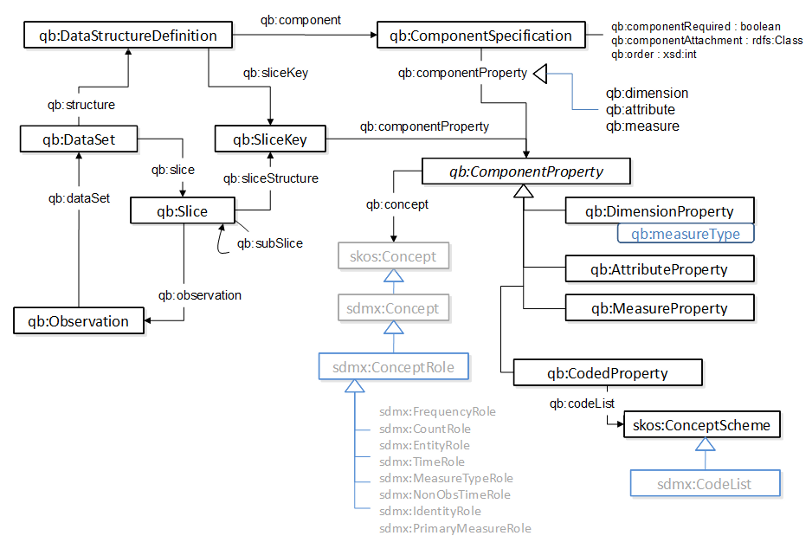
\includegraphics[width=14cm]{images/phd/qb-fig}
\caption{\textit{Outline of the RDF Data Cube vocabulary}.}
\label{fig:qb}
\end{figure}



\begin{figure}[!htp]
\begin{lstlisting} 
nomen-stats: sliceByRegionSex a qb:SliceKey;
  rdfs:label "Slice by region"@en;
  rdfs:comment "Fixed year, region and sex change"@en;
  qb:componentProperty
  nomen-stats:refPeriod; 
 .

nomen-stats: spopulation a
  qb:DataStructureDefinition;
  qb:component
    [qb:dimension nomen-stats:refPeriod; ],
    [qb:dimension nomen-stats:refArea; ],
    [qb:dimension sdmx-dimension:sex; ],
    [qb:measure
    nomen-stats:population; ];
qb:sliceKey nomen-stats: sliceByRegionSex .


nomen-stats:region/sex a qb:Slice;
  qb:sliceStructure
  nomen-stats: sliceByRegionSex;
  nomen-stats:refPeriod
  <http://reference.data.gov.uk/id/gregorian-interval/2010-01-01T00:00:00/P1Y> ;
  qb:observation
  nomen-obs:region/sex/m/53/08/02, ...
.

nomen-obs:region/sex/m/53/08/02 a qb:Observation;
  qb:dataSet nomen-stats:nomenclator2010;
  nomen-stats:refArea <http://purl.org/weso/nomenclator/asturias/2010/resource/53/08/02> ;
  nomen-stats:refPeriod <http://reference.data.gov.uk/doc/gregorian-interval/2010-01-01T00:00:00/P1Y> ;
  sdmx-dimension:sex sdmx-code:sex-M ;
  sdmx-attribute:unitMeasure <http://dbpedia.org/resource/Person>
  nomen-stats:population 17 ; 
.

\end{lstlisting}
	\caption{Ejemplo de \textit{Slice} en el \dataset RDF del Nomenclátor de Asturias 2010.}
	\label{fig:slice-nomen}
\end{figure}



\subsection{Tarea $t_{14}$-Infraestructura para \linkeddata}
La consecución de todos los procesos, métodos y tareas puede reflejarse en una infraestructura
de herramientas que proporcionen soporte desde dos puntos de vista:

\begin{description}
 \item [Completa.] Cubre todos los procesos, métodos y tareas suministrando las herramientas
adecuadas para cada uno de ellos. Los criterios de selección pueden variar dependiendo
del estado de madurez, de los datos a tratar, de las tareas a realizar, etc. En este sentido
la infraestructura definida en \textit{LOD2 project}, ver Sección~\ref{lod2-project}, se puede
considerar como paradigmática.
\item [Parcial.] Cubre alguno de los procesos, métodos o tareas. Por ejemplo, para el proceso
de publicación, se puede establecer una infraestructura especial que no tenga en cuenta ningún
otro proceso y de por hecho la existencia de datos. A continuación y siguiendo el ejemplo que se desarrolla a lo largo de este capítulo se advierte 
un modelo para para la publicación de datos, ver Figura~\ref{fig:deploy-nomenclator}, que 
supone la existencia de datos en un cierto repositorio y que no provee más operaciones
que la de acceso a datos sin realimentación.
\end{description}

El responsable de esta tarea será \textit{Desarrollador} y el \textit{Propietario de datos} que deberán
resolver de acuerdo a unas determinadas especificaciones el soporte a los datos. La especificación
de este despliegue puede ser una simple lista de componentes o el uso de diagramas UML particulares
para este tipo de procesos, como el diagrama de componentes o de despliegue.

\begin{figure}[!htb]
\centering
	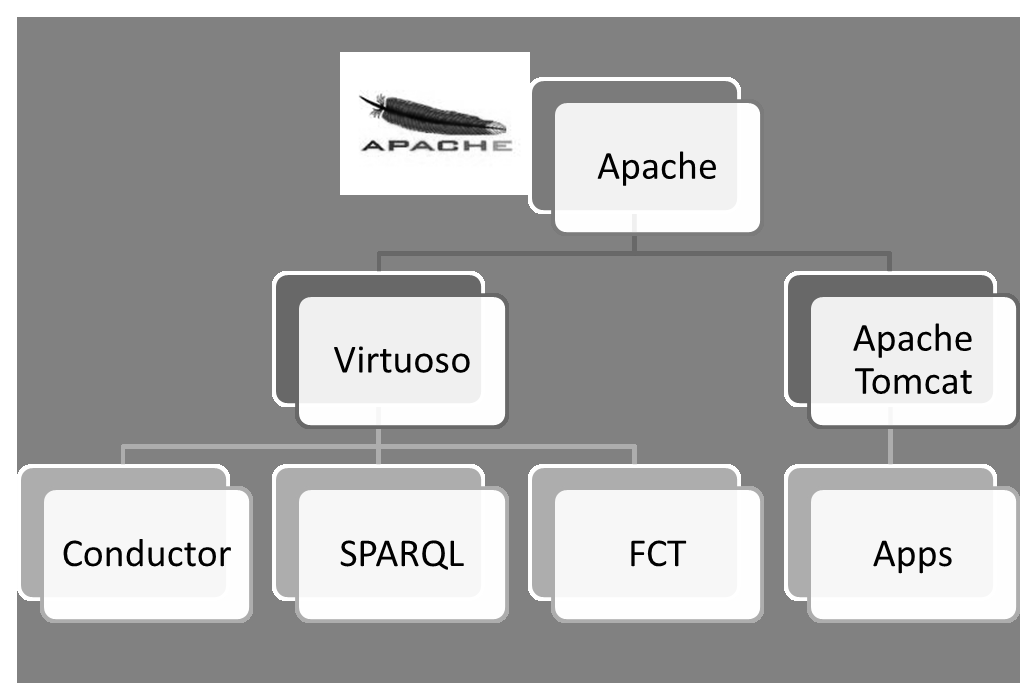
\includegraphics[width=12cm]{images/phd/infra-ld}
\caption{Infraestructura Parcial para el Nomenclátor de Asturias 2010.}
\label{fig:deploy-nomenclator}
\end{figure}

\subsection{Tarea $t_{15}$-Acceso y Formato de datos en RDF}
Seguidamente al proceso de generación de datos en RDF como \linkeddata es necesario establecer
los mecanismos de acceso a la información, en esta tarea se debe dar respuesta a una
serie de cuestiones:
\begin{itemize}
 \item ¿Cómo se va a desplegar la información?, ¿Fichero, repositorio, generación \textit{on-the-fly}, etc.?
 \item ¿En qué formatos se va a ofrecer esta información?
 \item ¿Qué tipo de acceso se va a permitir?, ¿Consulta directa a un \textit{endpoint} de \gls{SPARQL}?, ¿Un servicio web: \gls{REST}, \gls{SOAP}, etc.?
\end{itemize}

La responsabilidad de esta tarea recae en el \textit{Desarrollador} y el \textit{Propietario de datos} que han de decidir 
cómo se ha de hacer pública esta información de acuerdo a la estrategia de la entidad, de la infraestructura tecnológica y de los datos en sí mismos. 
El resultado de esta tarea debe proveer una especificación de cómo acceder a los datos en RDF y qué formatos se van a facilitar.

En el ejemplo que se está desarrollando, se ha decidido la siguiente estrategia:

\begin{itemize}
 \item Despliegue mediante un repositorio semántico con un \textit{endpoint} de \gls{SPARQL} habilitado y ficheros con los volcados completos de los datos.
 \item Los siguientes formatos deben ser prioritarios: \gls{HTML}, \gls{RDF/XML} y \gls{N3}.
 \item Acceso directo a consultar sobre el \textit{endpoint} de \gls{SPARQL} y un servicio de negociación de contenido sobre los datos.
\end{itemize}

\subsection{Tarea $t_{16}$-Añadir metainformación a los recursos RDF}\label{t16-metodos}
El objetivo de esta tarea es dotar a los recursos de información de la metainformación 
necesaria para suministrar soporte a la procedencia de los datos y garantizar 
un cierto grado de confianza en su uso. En esta tarea, existen dos enfoques 
posibles:
\begin{enumerate}
 \item Incluir la metainformación a nivel de \dataset. Esta opción se utilizará cuando 
los recursos tenga un carácter estático y evolucionen poco en el tiempo y en conjunto, de esta forma, 
tiene sentido incluir sólo metainformación a nivel del conjunto completo de datos para no generar 
información superflua.
 \item Incluir la metainformación a nivel de cada recurso. Este enfoque se utilizará cuando 
los recursos tengan un carácter dinámico y evolucionan en el tiempo independientemente de otros 
recursos en el conjunto de datos completo. 
 \item Enfoque híbrido. Evidentemente, si sólo algunos recursos del \dataset son candidatos 
a incluir metainformación a nivel de cada recurso es preferible optar por este enfoque facilitando 
la información donde sea necesaria. La principal desventaja de esta opción reside en que la transformación 
de los datos no es homogénea generando incertidumbre en los posibles clientes. 
\end{enumerate}

La responsabilidad de esta tarea recae en el \textit{Desarrollador} y el \textit{Propietario de datos} que han de decidir 
qué metainformación se debe incluir y qué enfoque aplicar. El resultado de esta tarea es el propio 
\dataset \gls{RDF} pero incluyendo nuevas tripletas para representar la información necesario como 
metadatos.

\subsection{Tarea $t_{17}$-Documentación extra}\label{t17-metodos}
Uno de los puntos clave para la reutilización de datos enlazados reside 
en la provisión de una documentación adecuado sobre qué tipo de recursos 
de información se han transformado y qué datos contienen. Desde un punto 
de vista estratégico las decisiones que se hayan tomado en cuanto a 
selección de vocabularios y otros \datasets a reutilizar ya supone 
una buena guía de documentación facilitando a los clientes datos 
perfectamente conocidos, ahora bien, desde una perspectiva 
operativa es conveniente documentar las decisiones tomadas como el diseño 
de URIs, el tipo de datos utilizado, el acceso a la información, las formas 
de consulta, posibles restricciones, etc. para que la selección del \dataset 
se convierte en una decisión sencilla. Un ejemplo claro de documentación correcta 
es la provista por \textit{GoodRelations} y \textit{ProductOntology} en las cuales 
además de los datos en sí mismos se ofrecen ejemplos de uso, características, casos 
de éxito en su reutilización, etc. favoreciendo su difusión entre la comunidad.

La responsabilidad de esta tarea recae en el \textit{Desarrollador} y el \textit{Propietario de datos} que han de establecer 
qué partes se pueden documentar públicamente y la forma de difundir la misma: mediante metadatos, etc. El resultado 
de esta tarea será, en general, una especificación de cómo se deben reutilizar los datos. En este sentido, en las últimas 
fechas ha habido una extensa discusión en la lista de correo de \lod en el \gls{W3C} sobre el uso de \texttt{HttpRange-14} para 
consultar cómo se debería incluir información de unos recursos en otros.

El resultado de esta tarea será una serie de documentos de especificación y ejemplos así como nuevas tripletas \gls{RDF} 
en el \dataset resultado para enlazar esta nueva metainformación.

\section{Proceso de Producción}\label{sect:produccion}

\begin{definition}[Producción]
Proceso que conlleva todas las tareas que implican la transformación de datos a un modelo RDF obteniendo 
como resultado un \dataset \gls{RDF} $\mathcal{D}$.
\end{definition}

\subsection{Método Semántico de Producción de \linkeddata}\label{method-prod-def}
\begin{definition}[Método Semántico de Producción]
$SPM$ es una función que para un conjunto de tuplas de entrada o \dataset $\mathcal{G}$ y un conjunto de \textit{mapeos} $\mathcal{M}$  
genera un \dataset RDF $\mathcal{D}$.
\end{definition}

\begin{center}
    $SPM : \mathcal{G} \times \mathcal{M} \longrightarrow \mathcal{D}$
\end{center}
Las características que tiene esta definición de un $SPM$ son las siguientes:
\begin{itemize}
 \item Para todo valor $f_{i}$ del conjunto de entrada $\mathcal{G}$, existe al menos un
\textit{mapeo} $m_{i}$ en el conjunto $\mathcal{M}$.
 \item Existen valores $f_{i}$ del conjunto de entrada $\mathcal{G}$, para los que existen
varios \textit{mapeos} $m_{i}$ formando un conjunto $\mathcal{M}_{i}$ subconjunto de $\mathcal{M}$.
\end{itemize}

Esta definición implica que toda la información de entrada permanece en el conjunto de salida. Si bien
se podría pensar que existen valores de la entrada, por ejemplo un identificador generado automáticamente desde
una base de datos, que no serían candidatos a persistir en el conjunto de salida es conveniente mantener
toda la información por la posibilidad de realizar realimentación y monitorización transversal. Si se apreciara 
la existencia de algún inconveniente con ocasión del consumo o de la publicación se deben proveer otros mecanismos para
hacer transparente esta información.

La interacción del proceso de producción de datos enlazados junto a otros procesos como el de publicación pueden
observarse en el diagrama, ver Figura~\ref{fig:produccion} realizado en \textit{Linked Data: Evolving the Web into a Global Data Space}~\cite{Heath_Bizer_2011} según
el cual se muestran algunos de los métodos utilizados para el proceso de producción de datos enlazados.

\begin{figure}[!htb]
\centering
	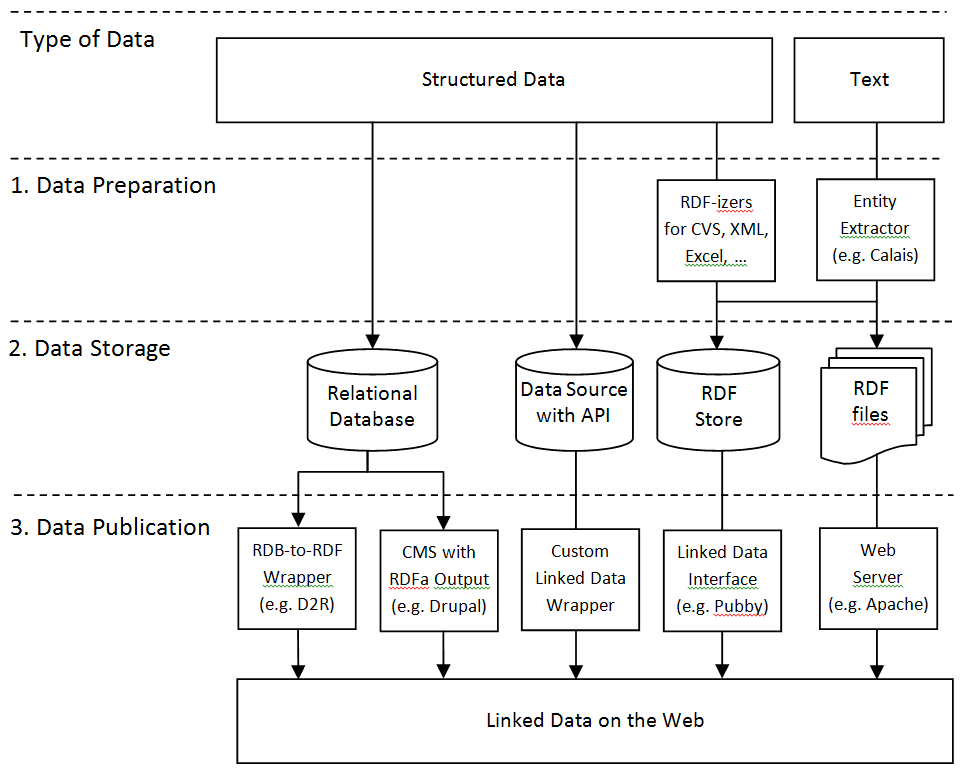
\includegraphics[width=10cm]{images/phd/linkeddata}
\caption{\textit{Linked Data Publishing Options and Workflows} (extraída de~\cite{Heath_Bizer_2011}).}
\label{fig:produccion}
\end{figure}


\subsection{$SPM_1$-Transformación de datos a RDF}\label{spm-1}
Este método de producción de un \dataset \gls{RDF}, $SPM_1$, asume que los datos disponibles se encuentran
en algún formato procesable automáticamente y que en cierto modo son estáticos o bien
es una imagen estática de los mismos. Se trata, en concreto del supuesto en el que se dispone de datos en formatos
como \gls{CSV} o MSExcel o bien se hace un volcado de una base de datos para generar posteriormente a partir
de estos valores de entrada el \dataset RDF. 

Por lo tanto, este enfoque se aplicará cuando nos encontremos en la siguiente situación:
\begin{itemize}
 \item Datos estáticos. Inicialmente sin disponibilidad de acceso mediante un lenguaje de consulta tipo \gls{XPath} o \gls{SQL}.
 \item Formato de datos preestablecido tipo CSV, MSExcel o \gls{XML}.
 \item El tamaño del \dataset de entrada no es excesivamente grande. No existe una forma de evaluar el tamaño
de un \dataset, pero se podría fijar que el resultado final fuera en orden de millones de tripletas RDF.
\end{itemize}


\subsection{$SPM_2$-\textit{Mapeo} con Base de Datos}\label{mapeo-bbdd}
Se trata de un método híbrido de producción y publicación de datos enlazados, $SPM_2$, que asume la existencia de una base de datos, en la mayoría de los casos
relacional, con datos preestablecidos a los cuales se puede acceder a través de un lenguaje de consulta
tipo \gls{XPath}, \gls{XQuery} o \gls{SQL}. Este procedimiento se fundamenta en la realización de un \textit{mapeo} con los datos
que se pretenden exportar como \gls{RDF} y la estructura de los mismos. Se pueden mezclar datos de diferentes tablas
y utilizar los lenguajes de consulta para generar datos agregados. Este enfoque se suele utilizar cuando
existe una gran base de datos de complejo volcado a ficheros y cuya transformación y posterior publicación
sería un proyecto de gran magnitud en sí mismo. Por lo tanto, se opta por una solución en la cual se utiliza una capa
intermedia que se encarga de acceder a los datos ya existentes y producir RDF bajo demanda. De esta forma,
se pueden reutilizar las bases de datos existentes, se considera un método no intrusivo ya que sólo requiere los
datos, pero puede provocar una sobrecarga en la actual base de datos, dada esta situación se suele optar por realizar
el envoltorio semántico sobre una imagen de la misma, así se protege la operatividad ordinaria mientras que se
da acceso mediante datos enlazados. La solución que propone este método debería utilizarse cuando el tamaño
de los datos es desmesurado y está en continua evolución, de tal manera que no es rentable realizar $SPM_1$ en
cada actualización de datos. La ventaja implícita reside precisamente en este último punto ya que se da soporte
directo a la actualización automática de la vista en RDF. 


Por lo tanto, este enfoque se aplicará cuando nos encontremos en la siguiente situación:
\begin{itemize}
 \item Datos dinámicos. Con posibilidad de acceso mediante un lenguaje de consulta tipo XPath o SQL.
 \item Modelo y formato de datos formal, por ejemplo basado en el Modelo Entidad/Relación.
 \item El tamaño del \dataset de entrada suele ser grande. El resultado final
estaría en el orden de billones de tripletas RDF.
\end{itemize}


\subsection{$SPM_3$-Consulta y transformación a RDF}
El método $SPM_3$ se utiliza cuando se cuenta con un sistema de gestión de datos al que se puede acceder 
a través de un lenguaje de consulta y que además de almacenar 
datos estrictamente, también contiene de otro tipo de información como texto. Este método se suele
utilizar en bases de datos documentales en las que la unidad de información es un 
documento con metadatos. Los datos promocionados a \linkeddata suelen incluir
la metainformación de los documentos esquivando la transformación de toda la información
con el objetivo de facilitar el acceso a los mismos. En resumen se provee acceso
a la metainformación que está estructurada mientras que los textos completos y libres, o bien no se promocionan o bien se ofrecen de forma completa 
sin análisis previo a través de otros vínculos.


Por lo tanto, este enfoque se aplicará cuando ante la siguiente situación:
\begin{itemize}
 \item Datos dinámicos, no posibilidad de acceso mediante un lenguaje de consulta tipo XPATH o SQL.
 \item Formato de datos preestablecido, sin embargo no tiene porque existir un modelo formal para los mismos.
 \item El tamaño del \dataset de entrada no debería ser relevante, simplemente se generan los datos en RDF bajo demanda.
\end{itemize}


\subsection{Tabla de Decisión del Proceso de Producción}
En resumen y considerando las tres variables siguientes: 1) evolución y actualización de los datos; 2) la existencia
de un modelo formal o acceso mediante lenguaje de consulta y 3) el tamaño del \dataset resultado, es factible establecer
la siguiente tabla de decisión, ver Tabla~\ref{tabla:produccion}.

\newpage

\begin{longtable}[c]{|p{1.3cm}|p{1.3cm}|p{1.6cm}|p{1.6cm}|p{1.3cm}|p{1.3cm}|p{1.3cm}|p{1.3cm}|p{1.3cm}|} 
\hline
 \multirow{2}{*}{\textbf{Método}} & \multicolumn{2}{|c|}{\textbf{Tipo}} & \multicolumn{2}{|c|}{\textbf{Formato}} &  \multicolumn{2}{|c|}{\textbf{Modelo Formal}} &  \multicolumn{2}{|c|}{\textbf{Tamaño Final}}\\ \cline{2-9} 
\endhead
	 & Estático & Dinámico & Estructura & Consulta & Si & No & Millones & Billones \\ \hline
 $SPM_1$ & $\star$  &  & $\star$ &  &  & $\star$ & $\star$ &  \\ \hline
 $SPM_2$ &   & $\star$  &  & $\star$ &  $\star$ &  &  & $\star$ \\ \hline
 $SPM_3$ &   & $\star$  & $\star$ & $\star$ &  $\star$ &  & $\star$  & $\star$ \\ \hline

\hline
\caption{Tabla de Decisión del Proceso de Producción de \linkeddata.}  \label{tabla:produccion} \\    
\end{longtable}

\section{Proceso de Publicación}\label{sect:publicacion}

\begin{definition}[Publicación]
Proceso que conlleva todas las tareas que implican el despliegue público de un \dataset \gls{RDF} $\mathcal{D}$.
\end{definition}

\subsection{Método Semántico de Publicación de \linkeddata}
\begin{definition}[Método Semántico de Publicación]
$S\mathcal{P}M$ es una función que para un \dataset RDF $\mathcal{D}$ y un conjunto de características
de publicación $\mathcal{P}$, obtiene como resultado un \dataset \gls{RDF} $\mathcal{D}_{pub}$ publicado cumpliendo $\mathcal{P}$.
\end{definition}

\begin{center}
    $S\mathcal{P}M :  \mathcal{D} \times \mathcal{P} \longrightarrow \mathcal{D}_{pub}$
\end{center}
Las características contenidas en esta definición de un $S\mathcal{P}M$ son las siguientes:
\begin{itemize}
 \item $\mathcal{D} \approxeq \mathcal{D}_{pub}$, ya que se pueden utilizar técnicas para
filtrar ciertos datos presentes en $\mathcal{D}$.
 \item El conjunto de características de publicación $\mathcal{P}$ se utilizan para la validación
de $\mathcal{D}_{pub}$.
 \end{itemize}

Esta definición de método semántico de publicación implica que para la existencia de datos en \gls{RDF} 
se establecen un conjunto de características que se deben cumplir en el momento de la publicación como
puede ser la negociación de contenido, \gls{URI}s referenciables, acceso mediante protocolos estándar como \gls{HTTP}, etc. El objetivo es proveer
un \dataset RDF que ofrezca las características necesarias para ser considerado
como \linkeddata, en este sentido se intenta que los datos publicados alcancen el nivel de 5 $\star$.

Adicionalmente, dependiendo del método seleccionado de publicación se debe proveer una infraestructura
de almacenamiento de los datos que puede ser un fichero, un repositorio RDF o una base de datos, de acuerdo al 
tipo seleccionado se podrán publicar los datos de una u otra forma. Si bien el proceso de almacenar
los datos generados puede estimarse como una tarea de producción o publicación, realmente se trata
de un proceso implícito, de ahí que el proceso de publicación sea dependiente del tipo de almacén 
utilizado. No obstante, existen soluciones que se combinan, por ejemplo se pueden publicar los datos
de un fichero RDF mediante un \textit{endpoint} de \gls{SPARQL} sin necesidad de disponer de un repositorio
RDF nativo, o bien se pueden utilizar extensiones de algunos sistemas de gestión de base de datos~\cite{oracle-rdf} 
que son capaces de manejar recursos RDF. La decisión sobre la solución que se deba adoptar, se tomará con ocasión 
del diseño de la infraestructura de \linkeddata que condicionará estratégicamente los procesos posteriores a la generación de los datos.

\subsection{$S\mathcal{P}M_{1}$-Fichero estático en RDF}\label{spm-1-pub}
Este método de publicación, $S\mathcal{P}M_{1}$, simplemente ofrece el conjunto de datos
a través de un fichero alojado en un servidor web y accesible mediante un protocolo estándar.
Es la forma de publicación que facilita en menor grado el acceso y reutilización de información, 
ya que para conseguir la descripción de cualquier recurso se debe obtener el \dataset completo 
con la consiguiente sobrecarga para su consumo posterior. Además es necesario configurar correctamente los 
tipos \gls{MIME} en el servidor web para que se ofrezca el contenido de modo adecuado.

La publicación de ficheros es una de las formas más utilizadas en multitud de circunstancias debido a su
sencillez, no requiere ningún tipo de infraestructura adicional, tanto desde el punto de vista de \opendata como de \linkeddata, ya que sólo requiere
hacer pública la información sin valorar otro tipo de consideraciones.

Por ejemplo, en el supuesto referido sobre el Nomenclátor de Asturias 2010 es posible habilitar en el servidor
web los volcados de los datos \gls{RDF} (serializados en \gls{N3}) en las siguientes \gls{URI}s:

\begin{itemize}
 \item <base\_uri> = \url{http://purl.org/weso/datasets/nomenclator/asturias/2010}
 \item <base\_uri>/nomenclator-asturias-2010.ttl
 \item <base\_uri>/nomenclator-asturias-2010-ontology.ttl
 \item <base\_uri>/stats/nomenclator-asturias-2010-stats.ttl
 \item <base\_uri>/stats/nomenclator-asturias-2010-stats-ontology.ttl
\end{itemize}

Además, se debe configurar en el servidor web, en este caso Apache2 fichero \texttt{/etc/mime.types}, 
cómo servir el tipo MIME con extensión ``ttl'' mediante la adición de la línea \texttt{text/turtle	ttl}. Como se puede
observar este método de publicación es el más básico y requiere la realización de configuración manual por no decir
la necesidad de verificar el correcto funcionamiento siguiendo las prácticas de publicación del W3C.

\subsection{$S\mathcal{P}M_{2}$-\textit{Mapeo} con Base de Datos}
Como se ha expuesto en la Sección~\ref{mapeo-bbdd} se trata de un método híbrido de producción
y publicación, $S\mathcal{P}M_{2}$, de datos enlazados. En este caso, los datos se generan bajo demanda mediante
una función de \textit{mapeo} entre la descripción \gls{RDF} que se debe producir y los datos
almacenados en la base de datos. En cuanto a la publicación, la descripción RDF se genera
bajo demanda atendiendo a las características prefijadas y es similar al caso que se presentará en la Sección~\ref{linkeddata-frontend} 
sobre la publicación con un \textit{Linked Data Frontend}, con la diferencia de que los datos no se hayan previamente en RDF sino 
que se generan dinámicamente.

\subsection{$S\mathcal{P}M_{3}$-\textit{Endpoint} de SPARQL}\label{spm-3-pub}
El uso de un \textit{endpoint} de \gls{SPARQL} está ampliamente asentado en la comunidad
de \linkeddata como método de publicación estándar, $S\mathcal{P}M_{3}$, mediante
el cual además de publicar la información de los recursos RDF, se ofrece un servicio
de consulta mediante el lenguaje SPARQL. Este método de publicación requiere
el uso de un repositorio \gls{RDF} en el cual se almacenan los datos RDF previamente
transformados por lo que es incompatible con los métodos de generación de RDF bajo demanda.

La aplicación de este método de publicación es la más interesante desde el punto de vista
de la reutilización ya que permite la creación y ejecución de consultas sobre los datos RDF por lo que
se pueden consolidar aquellos previamente no generados. Desde un punto de vista tecnológico requiere
de infraestructura adicional ya que es necesario disponer de un repositorio RDF dotado de un servicio SPARQL.

\subsection{$S\mathcal{P}M_{4}$-\textit{On-the-fly}}
Al igual que en el método de publicación desde una base de datos, se trata de un método híbrido
de generación y publicación de datos enlazados bajo demanda, $S\mathcal{P}M_{4}$. Las descripciones en \gls{RDF} de los
recursos no existen físicamente sino que se generan bajo petición. Resulta interesante cuando
el publicador de datos es diferente del propietario de datos y también para ofrecer
dinámicamente una capa de datos enlazados sobre servicios preexistentes, pese a que la generación
y publicación se realiza bajo demanda, en ningún caso se obvian las tareas implicadas en estos procesos.

Este método es el utilizado en servicios como RDFohloh~\cite{Ferndez08rdfohloh} para generar y publicar la información
sobre los proyectos disponibles en el portal Ohloh~\cite{ohloh}. Por ejemplo, ver Figura~\ref{fig:moldeas-ohloh}, se puede obtener la descripción
del proyecto \gls{MOLDEAS} en las siguientes \gls{URI}s y bajo las mismas características que se definirían en otros métodos como la negociación de contenido, etc.:
\begin{itemize}
 \item \url{http://rdfohloh.wikier.org/project/moldeas/html}
 \item \url{http://rdfohloh.wikier.org/project/moldeas/rdf}
 \item \url{http://rdfohloh.wikier.org/project/moldeas/n3}
 \item \ldots
\end{itemize}


\begin{figure}[!htp]
\begin{lstlisting}

<http://rdfohloh.wikier.org/project/moldeas/rdf> dct:isFormatOf 
	<http://rdfohloh.wikier.org/project/moldeas>;
	a foaf:Document;
	rdfs:label "MOLDEAS's DOAP document serialized in RDF/XML";
	foaf:primaryTopic <http://rdfohloh.wikier.org/project/moldeas>.
	<http://rdfohloh.wikier.org/project/moldeas> dct:updated "2011-12-25T10:04:51Z";
	rdfohloh:ohloh-page <http://www.ohloh.net/projects/moldeas>;
	doap:created "2011-10-14T09:19:11Z";
	doap:description "This work aims to apply the semantic web and LOD approaches to public procurement notices...";
	doap:download-page <http://code.google.com/p/moldeas/downloads/list>;
	doap:homepage <http://purl.org/weso/moldeas/>;
	doap:name "MOLDEAS";
	doap:programming-language "JavaScript";
	a doap:Project;
	= <http://rdfohloh.wikier.org/project/586667>;
	skos:subject <http://dbpedia.org/resource/JavaScript>.

\end{lstlisting}
	\caption{Ejemplo de generación \textit{On-the-fly} de \linkeddata.}
	\label{fig:moldeas-ohloh}
\end{figure}

\subsection{$S\mathcal{P}M_{5}$-\linkeddata \textit{Frontend}}\label{linkeddata-frontend}
La evolución en los métodos de publicación derivada de la necesidad de cumplir
con los criterios de \linkeddata ha motivado la creación de herramientas
que proporcionen soporte a los mismos. De esta manera, ha surgido tecnología tal como
los \linkeddata \textit{Frontend}, $S\mathcal{P}M_{5}$, que simplifican el método de publicación
realizando de forma automática muchas de las tareas que antes se realizaban manualmente y que sirven para cumplir con las características de publicación $\mathcal{P}$, 
como la negociación de contenido, el uso de HTTP URIs, etc. Se puede considerar
la evolución natural de la reescritura de URLs, que se utilizaba previamente, la cual requería un profundo conocimiento 
de los módulos de reescritura de los servidores web.

No obstante, este método de publicación se basa en la existencia de un \textit{endpoint}
en \gls{SPARQL}, sobre el que se puedan ejecutar consultas \textit{DESCRIBE}. El funcionamiento del mismo 
consiste en la extracción e identificación de la \gls{URI} del recurso y teniendo en cuenta $\mathcal{P}$ generar 
una representación del mismo preguntando al repositorio \gls{RDF}. 

La principal ventaja de este método reside en la configuración del mismo, suficientemente informe, se puede
realizar para cada uno de los \dataset RDF disponibles en un repositorio obteniendo
de forma sencilla el acceso a los recursos RDF. Además, este método no resulta intrusivo
con las herramientas de almacenaje de RDF, ya que son aplicaciones externas añadidas como una capa nueva de acceso para facilitar 
la publicación y el consumo.

Por ejemplo, utilizando \gls{Pubby} y una configuración, ver Figura~\ref{fig:nomen-pubby}, se puede 
publicar la información del Nomenclátor de Asturias 2010 que previamente ha sido almacenada
en un repositorio RDF.

\begin{figure}[!htp]
\begin{lstlisting}

<> a conf:Configuration;
    conf:projectName "Nomen 2010 Asturias";
    conf:projectHomepage <http://purl.org/weso/nomenclator/>;
    conf:webBase <http://purl.org/weso/nomenclator/>;
    conf:usePrefixesFrom <>;
    conf:defaultLanguage "en";
    conf:indexResource 
      <http://purl.org/weso/nomenclator/asturias/2010/resource/ds>;

conf:dataset [
        conf:sparqlEndpoint <http://156.35.31.156/sparql>;
        conf:sparqlDefaultGraph <http://purl.org/weso/nomenclator/asturias/2010>;
        conf:datasetBase <http://purl.org/weso/nomenclator/>;
        conf:datasetURIPattern "asturias/2010/resource/.*";
        conf:webResourcePrefix "";
        conf:fixUnescapedCharacters "(),'!$&*+;=@";
	conf:metadataTemplate "metadata.ttl";
	meta:pubbyUser <http://purl.org/weso>;
        meta:pubbyOperator <http://purl.org/weso>;
];
conf:dataset [
	conf:sparqlEndpoint <http://156.35.31.156/sparql>;
	conf:sparqlDefaultGraph <http://purl.org/weso/nomenclator/ontology>;
        conf:datasetBase <http://purl.org/weso/nomenclator/>;
        conf:datasetURIPattern "ontology/.*";
	conf:webResourcePrefix "";
	conf:fixUnescapedCharacters "(),'!$&*+;=@";
	...
    ];

conf:dataset [
       conf:sparqlEndpoint <http://156.35.31.156/sparql>;
       conf:sparqlDefaultGraph <http://purl.org/weso/nomenclator/asturias/2010/stats>;
       conf:datasetBase <http://purl.org/weso/nomenclator/>;
       conf:datasetURIPattern "asturias/2010/stats/resource/.*";
       conf:webResourcePrefix "";
       conf:fixUnescapedCharacters "(),'!$&*+;=@";
        ....
 ];
.
\end{lstlisting}
	\caption{Ejemplo de configuración de Pubby para el Nomenclátor de Asturias 2010.}
	\label{fig:nomen-pubby}
\end{figure}


\subsection{$S\mathcal{P}M_{6}$-Servicio Web}\label{servicio-web-produccion}
Este método de publicación, $S\mathcal{P}M_{6}$, se puede considerar un híbrido
entre los citados anteriormente, ya que en realidad un \linkeddata \textit{Frontend} es en esencia 
un servicio web dotado de ciertas características que permiten el acceso mediante URIs definidas a los contenidos
que se generan y publican en un repositorio \gls{RDF}. También un servicio web puede generar las descripciones
RDF bajo demanda, o bien constituir un envoltorio sobre una petición a una base de datos obteniendo
la representación de los datos en RDF. En general, este es el método de publicación más abierto, 
ya que la fuente de los datos en RDF puede ser variada: fichero estático, repositorio, bajo demanda, etc., 
y la publicación se puede basar en: generación bajo demanda, consultas, etc. Habitualmente se utilizarán
servicios bajo el modelo \gls{REST} por su complicidad respecto a la iniciativa \linkeddata, también sería posible invocar servicios 
bajo el protocolo \gls{SOAP} incluyendo las representaciones RDF en el cuerpo de la respuesta del servicio. 


\subsection{Privacidad en la Publicación de \linkeddata}
El concepto de privacidad en los datos enlazados se pone de manifiesto en el momento
en el que existe información y datos dependiendo de ciertos factores deben ser filtrados, como por ejemplo el tipo
de usuario. Desde una perspectiva conceptual la publicación de datos
enlazados puede verse sometida a cuestiones de privacidad, pero no así refiriéndose 
a \opendata o \lod, en los cuales no se debería someter los datos a ningún tipo de filtro
con el objetivo de facilitar la transparencia. No obstante, es conveniente sopesar 
como parte de la publicación de datos la posibilidad de establecer vistas
o filtros que puedan agregar la información bien para su consumo o por cuestiones
legales, actualmente, la forma de obtención de esta característica desde la iniciativa
de \linkeddata se puede realizar mediante la generación de vistas en \gls{RDF}:

\begin{itemize}
 \item Usar grafos nombrados, en los cuales sólo estén disponibles los datos que se deseen públicos, evidentemente,
si todos los datos están publicados en un \textit{endpoint} de \gls{SPARQL}, sortear esta restricción no supone un gran inconveniente.
\item Filtrar ciertos valores o relaciones en las consultas sobre los datos publicados.
\item Definir usuarios, roles, listas de control de acceso sobre los datos publicados y los grafos.
\end{itemize}

Sin duda la privacidad no es concepto nuevo, ya que las bases de datos tradicionales incluyen el concepto
de \textit{vista} para ofrecer soporte a este tipo de característica. En cualquier caso, esta cuestión no ha sido abordada
completamente desde el punto de vista de la ingeniería y como ya se ha comentado se emplean soluciones parciales
reutilizando la tecnología semántica. La forma más coherente y elegante de adoptar la privacidad como característica
de la publicación de datos sería seguir un enfoque parecido a los \linkeddata \textit{Frontends}, pero aún no se ha contemplado como un propósito estratégico.

\section{Proceso de Consumo}

\begin{definition}[Consumo]
Proceso que conlleva todas las tareas que implican el acceso a los recursos de un \dataset \gls{RDF} $\mathcal{D}_{pub}$.
\end{definition}


\subsection{Método Semántico de Consumo de \linkeddata}\label{sect:proceso-consumo}
\begin{definition}[Método Semántico de Consumo]
$SCM$ es una función que para un \dataset RDF $\mathcal{D}_{pub}$, con unas características de publicación $\mathcal{P}$ y un conjunto de \textit{mapeos}
$\mathcal{M}^1$, obtiene como resultado la representación de los recursos $r_k \in \mathcal{D}_{pub}$ en otro modelo formal.
\end{definition}

\begin{center}
    $SCM :  \mathcal{D}_{pub} \times \mathcal{M}^1 \longrightarrow \mathcal{D}_{consum}$
\end{center}
Las características que tiene esta definición de un $SCM$ son las siguientes:
\begin{itemize}
 \item $\mathcal{D}_{pub}$ no es modificado por los métodos de consumo.
 \item $\mathcal{P}$ indica como se accede al \dataset \gls{RDF}.
 \item $\mathcal{M}^1$ indica como transformar el \dataset $\mathcal{D}_{pub}$ a la representación objetivo.
 \end{itemize}

Esta definición de consumo implica por un lado, que los datos se pueden consumir directamente para realizar operaciones
como navegación y representación gráfica o que se pueden utilizar para cargar valores dentro de objetos
de un lenguaje de programación formando parte de la lógica de negocio de una aplicación.

\subsection{$SCM_1$-Directo de datos en RDF}
Este método de consumo, $SCM_1$ está ampliamente asentado para la creación de aplicaciones
que simplemente realicen una visualización, navegación o creación de \textit{mashups} con los
datos publicados. Es la forma más sencilla de consumo y encaja impecablemente con el concepto
de Web 2.0, en el cual se consumen distintas fuentes de datos, servicios o APIs de distintos
proveedores para generar un servicio agregado en el cual poder manejar los datos. La lógica
de negocio de estas aplicaciones suele ser relativamente simple ya que las operaciones a realizar
con los datos no trascienden de la mera agregación e integración de varias fuentes de datos.

Actualmente es considerable la relevancia que están adquiriendo este tipo de aplicaciones y de ahí que la representación 
de \gls{RDF} en \gls{JSON} haya logrado una gran trascendencia con el objetivo de facilitar a los desarrolladores, procedentes desde ámbitos ajenos a la Web Semántica, 
la reutilización de datos enlazados.

Por otra parte, los sistemas de visualización de datos están ampliamente asentados y existen
múltiples herramientas que permiten la presentación de los mismos. La tendencia actual en este
tipo de consumo se centra en el enriquecimiento automático y bajo demanda de los datos disponibles: descubriendo
nuevos \datasets, enriqueciendo la información textual con elementos multimedia o georreferenciación, etc.


\subsection{$SCM_2$-\textit{Mapeo} a Lenguaje de Programación}\label{scm2-consumo}
Tradicionalmente el acceso a datos ha sido una de las partes clave en el desarrollo de aplicaciones con el objetivo
de asegurar la persistencia de los objetos de negocio y recuperarlos de forma sencilla. El uso de sistemas de bases de datos relacionales
requería una transformación del Modelo Entidad/Relación a un modelo orientado a objetos, estructurado, funcional o basado
en prototipos dependiendo del lenguaje de programación y del paradigma utilizado en el cual se realizaba mediante
una serie de \textit{mapeos} que permitían ``cargar'' los objetos de negocio con valores procedentes de la base de datos.
La diversidad de datos y la heterogeneidad en los modelos de representación ha comportado a la proliferación 
de herramientas que facilitan el \textit{mapeo} entre distintas entidades, por ejemplo el uso de ORMs como Hibernate o Linq en los lenguajes
orientados a objetos está ampliamente asentado. En el caso que nos ocupa, $SCM_2$, surge una situación similar en la que
se dispone de un modelo fuente para la representación de los datos, RDF, y un modelo objetivo que puede ser
que depende del paradigma en el que estemos programando. En este escenario se manifiesta la necesidad
de disponer de un tipo de \gls{ORM} para combinar \gls{RDF} con los objetos de negocio, etc., de un lenguaje de programación, pero 
la realidad es que todavía no se ofrecen herramientas que permitan realizar este promoción de los datos enlazados
a objetos de nuestra lógica de negocio de una forma sencilla. Los enfoques que se suelen seguir son los siguientes:

\begin{enumerate}
 \item Programar manualmente los accesos a datos mediante consultas \gls{SPARQL} o un \gls{API} RDF para crear
nuestros objetos de negocio con los datos previos en RDF.
\item \textit{Mapeo} semi-automático indicando a las propiedades de nuestro modelo objetivo con qué propiedades
del \dataset RDF se deben cargar.
\item Transformación automática de ontologías a un modelo de un lenguaje de programación y en consecuencia
a partir de los recursos RDF que sean instancias de esa ontología crear instancias del modelo objetivo.
\end{enumerate}

Este tipo de enfoques para el consumo de datos han sido estudiados en el proyecto \gls{TRIOO}~\cite{DBLP:conf/icsoft/FernandezBRG10} lo que ocurre 
verdaderamente es que se sigue abordando el problema desde un enfoque en gran medida manual, con el consecuente perjuicio para las 
aplicaciones que consuman datos enlazados.

\section{Proceso de Validación}\label{sect:validation}
\begin{definition}[Método Semántico de Validación]
$SVM$ es una función que para un \dataset \gls{RDF} $\mathcal{D}$ y un conjunto de características
a validar $\mathcal{V}$, obtiene como resultado un conjunto de aserciones $\mathcal{A}$.
\end{definition}

\begin{center}
    $SVM :  \mathcal{D} \times \mathcal{V} \longrightarrow \mathcal{A}$
\end{center}
Las características que tiene esta definición de un $S\mathcal{P}M$  son las siguientes:
\begin{itemize}
 \item El \dataset RDF $\mathcal{D}$ no es modificado durante el proceso de validación.
 \item El conjunto de características a validar $\mathcal{V}$ depende del proceso
que deseemos contrastar.
 \item El conjunto de aserciones obtenidas tras el proceso de validación $\mathcal{A}$, indica el grado de cumplimiento de $\mathcal{D}$ de acuerdo a $\mathcal{V}$.
 \end{itemize}

La validación de los datos enlazados es aplicable a todos los procesos del ciclo de vida, de esta manera,
se aseguran tanto características de calidad como principios de \linkeddata, \opendata y \lod, validación
de enlaces, etc. 

El proceso de validación se puede realizar de dos formas:
\begin{description}
 \item [Manual.] Mediante la revisión personal de las características deseables para cada uno de los recursos del \dataset RDF $\mathcal{D}$.
 \item [Automática.] Mediante el uso de herramientas existentes que permiten verificar ciertas características de los datos enlazados, por ejemplo 
el validador Vapour~\cite{Berrueta08cookinghttp} o el presente para la publicación de \datasets en la nube de \linkeddata.
\end{description}

El uso de recursos ``plantilla'' o ejemplos en la metainformación de un \dataset RDF ayuda a la realización de 
los procesos de validación ya que permite extraer ciertas características
que han de cumplir todos los recursos pertenecientes a un \dataset determinado. No obstante,
la validación de datos enlazados todavía no ha tenido un impulso enérgico por parte
de la comunidad, por lo que el método más utilizado es la validación manual. Esta situación
tiene como principal ventaja que se promueve la publicación masiva de datos sin poseer grandes barreras de entrada, sin embargo presenta como inconveniente la obtención 
de un entorno de datos en el que la incertidumbre sobre la calidad de los mismos o su consumo carece de respaldo. 
La tendencia en este tipo de proceso lleva a la convergencia hacia iniciativas ya asentadas, 
como las de accesibilidad web en la cual se tienen una serie de perfiles con un grado de cumplimiento de reglas que permiten asegurar que las páginas web cumplen ciertos
requisitos. 


\section{Proceso de Realimentación}\label{proceso-realimentacion}
\begin{definition}[Realimentación]
Proceso que conlleva todas las tareas que implican la actualización de \datasets \gls{RDF} preexistentes, se trata de una agregación de los procesos anteriores.
\end{definition}

\begin{definition}[Método Semántico de Realimentación]
$SFM$ es una función que para un \dataset RDF $\mathcal{D}$ publicado como $\mathcal{D}_{pub}$ y un conjunto de relaciones y 
valores a modificar $\mathcal{RV}$, obtiene como resultado un nuevo \dataset RDF $\mathcal{D}'$ que se publica como $\mathcal{D}'_{pub}$.
\end{definition}

\begin{center}
    $SFM :  \mathcal{D}_{pub} \times \mathcal{RV} \longrightarrow \mathcal{D}'$
\end{center}
Las características que tiene esta definición de un $SFM$  son las siguientes:
\begin{itemize}
 \item El \dataset RDF publicado $\mathcal{D}'$, se considera un nuevo conjunto
de datos diferente a $\mathcal{D}_{pub}$.
 \item El \dataset RDF $\mathcal{D}$, sólo se modifica en la parte de datos
que se haya publicado como $\mathcal{D}_{pub}$. En la mayoría de los casos $\mathcal{D}_{pub} \approxeq \mathcal{D}$, por lo
que la definición se puede extender fácilmente a $\mathcal{D}$.
 \item El conjunto de relaciones y valores a modificar $\mathcal{RV}$ es un conjunto de tripletas
de la forma $<r_k,p,v>$, donde $r_k$ es un recurso del \dataset $\mathcal{D}_{pub}$, $p$ es una relación
presente en el recurso $r_k$ y $v$ es el valor de la relación $p$ en $r_k$. Además de actualizar
relaciones y valores existentes también puede implicar la adición o borrado de una tripleta $<r_k,p,v>$.
 \item El cambio en los valores de las tripletas de un recurso puede implicar cambios en el modelo
formal $\mathcal{O}$ de los recursos.
 \item Esta definición puede exigir cambios en el proceso de generación y publicación ya que dependiendo
del método utilizado estas actualizaciones deben ser almacenadas.
 \end{itemize}

El método de realimentación se interpreta como una composición de los métodos producción, consumo y publicación, ya que 
tanto si se modifican tripletas existentes (en cuanto a valores) como si se añaden o borran tripletas de los recursos, 
puede ser necesario ejecutar los métodos anteriores de forma completa, se asume que:
\begin{itemize}
 \item $\mathcal{M}$ es el conjunto de \textit{mapeos} para la producción de un \dataset.
 \item $\mathcal{P}$ es el  conjunto de características de publicación.
 \item $\mathcal{M}^1$ es el conjunto de \textit{mapeos} para el consumo de datos.
 \item $\mathcal{M}^1 = \mathcal{RV} $.
 \item $\mathcal{D}'_{pub}$ es el \dataset RDF $\mathcal{D}'$ publicado, tras aplicar el método de realimentación.
\end{itemize}

por tanto, la composición de los métodos ya definidos de consumo ($SCM$), producción ($SPM$) y publicación ($S\mathcal{P}M$) deben generar un
nuevo \dataset RDF publicado como $\mathcal{D}'_{pub}$.

\begin{align}
S\mathcal{P}M \circ SPM \circ SCM (\mathcal{D}_{pub}, \mathcal{RV}) \equiv \mathcal{D}'_{pub} \\
S\mathcal{P}M \circ SPM \circ SCM (\mathcal{D}_{pub}, \mathcal{M}^1) \equiv \mathcal{D}'_{pub} \\
S\mathcal{P}M \circ SPM (\mathcal{D}_{consum}, \mathcal{M}) = \mathcal{D}'_{pub} \\
S\mathcal{P}M (\mathcal{D}', \mathcal{P}) = \mathcal{D}'_{pub} \\
\mathcal{D}'_{pub} = \mathcal{D}'_{pub}
\end{align}

Así, atendiendo a las definiciones de los métodos semánticos realizadas, el proceso de realimentación
se puede formular como una composición de los procesos de consumo, producción y publicación.

\begin{center}
$S\mathcal{P}M \circ SPM \circ SCM (\mathcal{D}_{pub}, \mathcal{RV}) \equiv SFM (\mathcal{D}_{pub}, \mathcal{RV}) $:
\end{center}

\subsection{Lenguaje de Actualización}\label{sect:sparul}
Si el método de publicación utilizado es un \textit{endpoint} de SPARQL sobre
un repositorio RDF con capacidades para \gls{SPARUL} o \gls{SPARQL} 1.1, entonces
se pueden actualizar tripletas y recursos RDF mediante el propio lenguaje
de consulta SPARQL con las nuevas características de actualización. Este método
resulta sin duda el más apropiado, ya que es declarativo y se puede utilizar
toda la potencia del lenguaje de consulta para seleccionar y actualizar
aquellos recursos que se obtengan como respuesta.

Por ejemplo utilizando la consola de Virtuoso de OpenLink se pueden ejecutar
este tipo de sentencias, ver Figura~\ref{fig:sparul}, (borrar e insertar una tripleta RDF 
en un grafo nombrado):

\begin{figure}[!htp]
\begin{lstlisting}
SPARQL DELETE FROM GRAPH <http://purl.org/weso/pscs/isic/v4> { ?s void:dataDump  ?o }  
  FROM <http://purl.org/weso/pscs/isic/v4> WHERE {  
      ?s  void:dataDump  ?o  
    };

SPARQL INSERT INTO GRAPH <http://purl.org/weso/pscs/isic/v4> { 
  <http://purl.org/weso/pscs/isic/v4/resource/ds> void:dataDump 
    <http://purl.org/weso/datasets/pscs/isic/v4/isic-v4.ttl> 
  };
\end{lstlisting}
	\caption{Ejemplo de uso de un lenguaje de actualización .}
	\label{fig:sparul}
\end{figure}


\subsection{Descubrimiento Automático}\label{sect:desc-auto}
Un método de actualización se puede implementar a través de un proceso 
continuo en el que una vez actualizados los datos se ejecute la combinación
de los métodos de consumo, producción y publicación. En este caso, la actualización
es un \textit{workflow} automático que puede ser inducido por cambios en una base
de datos o por manifestarse nuevas relaciones en \datasets que se hayan publicado
posteriormente. En el primero de los casos, la estructura y definición de los recursos
no debería variar, ya que se trata de una nueva remesa de datos pero con la misma estructura, 
rangos y dominios para las propiedades y valores. Por ejemplo en el caso de información
de sensores se actualiza constantemente pero los valores tomados y su paso por el proceso
de producción y publicación es siempre el mismo. En el segundo caso tras estimar o
descubrir la posibilidad de alterar el \dataset publicado se añaden nuevas propiedades
o valores, lo que puede implicar la necesidad de cambiar el modelo formal para que
sea consecuente con los valores representados. Un ejemplo de este segundo caso, sería cuando se añaden referencias a otros \datasets de forma automática utilizando
las propiedades léxicas de los recursos previos.
\subsection{Actualización Ocasional}
En este caso se corrigen valores del \dataset \gls{RDF} publicado en recursos concretos y que no 
se hayan detectado durante las fases de validación, es un escenario de refinamiento por el uso
de los datos con el objetivo de verificar su calidad y validez. Por ejemplo tratando con 
valores a nivel internacional para publicar datos económicos, puede ser que el separador
utilizado para los ``miles'' no esté unificado en todos los casos, el hallazgo de 
un recurso con un valor ``extraño'' da lugar a su cambio sin alterar a otros datos
y recursos presentes en el \dataset.
\subsection{Actualización Incremental}
Este método de actualización surge por la necesidad de un refinamiento progresivo
al manifestarse nuevas necesidades en la descripción de los recursos, para que tengan
en cuenta más información. La forma de proceder puede ser automática, ver Sección~\ref{sect:desc-auto}, o 
bien manual añadiendo más datos en un determinado tipo de recurso.
\subsection{Usuarios y Aplicaciones}
En la mayoría de los casos la actualización y cambios en los datos enlazados son controlados
por el \textit{Desarrollador} o el \textit{Propietario de datos}. Dependiendo de la naturaleza, licencia
de uso y nivel crítico de los mismos, se puede habilitar la edición para terceros como 
usuarios y aplicaciones. Actualmente este enfoque no se ha extendido ya que en definitiva 
requiere la validación por parte del \textit{Propietario de datos}, pero contribuiría enormemente 
a realimentar los conjuntos de datos publicados. Un enfoque similar consiste en consultar a los usuarios finales qué datos les gustaría
tener disponibles, pero en ningún caso se permite una especie de \textit{crowdsourcing} de datos
enlazados. También en aquellos enfoques en los que se genera \gls{RDF} bajo demanda transformando
datos de un sitio o servicio web, se podrían actualizar los datos de la fuente, por ejemplo
en OhLoh disponiendo de los permisos de usuario adecuados se podría modificar la la información 
que después aparece en la versión RDF.

\section{Tablas de Validación}\label{sect:tablas-validacion}
El objetivo de esta sección es definir una serie de características 
en el ámbito de \linkeddata, \opendata y \lod que sirvan para verificar que
la aplicación de los métodos semánticos es correcta y con ello obtener
datos enlazados que aporten las ventajas conocidas sobre el uso
de esta iniciativa. De esta manera, si se consigue asegurar que los datos
producidos mediante estos métodos semánticos concuerdan con las directrices marcadas, se puede confirmar la calidad en los datos, impulsar la reutilización de los mismos y
mejorar consecuentemente el acceso a la información que conllevan. Una vez
que se apliquen estos métodos a un determinado dominio, como el de las licitaciones públicas, se disponen de estas tablas como método de validación. 

La elaboración de estas tablas surge de la agregación de varias fuentes:
\begin{enumerate}
 \item Principios de \linkeddata~\cite{Berners-Lee-2006}.
 \item Principios de \opendata~\cite{okfn} . 
 \item Especificaciones y documentos del \gls{W3C} como~\cite{publishing-ogd,linked-data-cookbook,Berr08}. 
 \item \textit{Linked Data Design Considerations} del libro \textit{Linked Data: Evolving the Web into a Global Data Space}~\cite{Heath_Bizer_2011}.
 \item \textit{Linked Data Patterns}~\cite{linked-data-patterns}.
 \item ``\textit{Basic Profile Resources}''~\cite{basic-profile-ibm} de IBM.
 \item Principios para incluir \datasets en la nube de datos enlazados y añadir al registro de \gls{CKAN}~\cite{ckanValidator}.
 \item Documentación específica, ver Sección~\ref{linked-data-spec}.
 \item Experiencia adquirida.
\end{enumerate}

La forma en las que se modelan estas tablas es la de un cuestionario de manera que la evaluación de una característica puede tener las siguientes respuestas:
\begin{description}
 \item [Positiva \si.] La característica es aplicable y se ha realizado en el actual \dataset.
 \item [Negativa \no.] La característica es aplicable y no se ha realizado en el actual \dataset.
 \item [No aplicable \na.] La característica no es aplicable y no se ha realizado en el actual \dataset.
\end{description}

Las tablas que se presentan en las siguientes secciones, cuya descripción completa se haya en el Apéndice~\ref{capitulo:tablas}, permiten verificar los siguientes
procesos, métodos semánticos, principios, patrones de diseño y características para difundir los \datasets \gls{RDF}:

\begin{enumerate}
 \item La Tabla~\ref{table:produccion-validator}, con identificador $T^{1}$, realiza una validación de las características, en total $69$, 
propias de los procesos de producción y publicación. La validación del proceso de consumo vendrá
determinada por la viabilidad de los dos anteriores. De la misma forma el proceso de realimentación
como composición de los anteriores se puede verificar mediante las cuestiones planteadas en esta tabla.
\item La Tabla~\ref{table:linkeddata-patterns}, con identificador $T^{2}$, presente en la Sección~\ref{linked-data-patterns} señala los patrones de diseño 
aplicados, en total $44$, utilizados para el modelado de datos.
\item La Tabla~\ref{tabla:linked-data}, con identificador $T^{3}$, presente en la Sección~\ref{def-linkeddata} indica el grado
de cumplimiento de los principios de \linkeddata y del Modelo de 5 $\star$, en total $4+5$, esta tabla se ha dividido para suministrar 
una información más adecuada.
\item La Tabla~\ref{tabla:open-data}, con identificador $T^{4}$, indica el grado
de cumplimiento de los principios de \opendata, en total $8+14$, esta tabla se ha dividido para suministrar una información 
más adecuada.
\item La Tabla~\ref{tabla:lod-cloud}, con identificador $T^{5}$, indica el grado de cumplimiento de los principios, en total $5$, para formar parte
del diagrama ``Linking Open Data Cloud''.
\item La Tabla~\ref{tabla:ckan}, con identificador $T^{6}$, indica el grado de cumplimiento de los principios, en total $47$, para formar parte
de un registro de \datasets basado en \gls{CKAN}.
\end{enumerate}

Obviamente, el cumplimiento de ciertas preguntas, principios o directrices conlleva el de 
otros presentes en las diferentes tablas. No obstante, es conveniente separar estas características
para efectuar la evaluación del nivel en el que se encuentra un \dataset.

 
\subsection{Tabla de Validación de los Procesos y Métodos Semánticos}

En la Tabla~\ref{table:produccion-validator} se realiza un cuestionario con una posible descripción
de la pregunta a realizar en el momento de la evaluación de los procesos y métodos semánticos, han sido agrupadas ya que algunas pueden ser tomadas 
desde distintos puntos de vista y enclavadas en diferentes procesos y métodos, por ejemplo ``¿Las URIs utilizadas permiten acceder a los recursos?'', sería
una característica a asegurar en el proceso de producción y publicación.

\begin{longtable}[c]{|l|p{8cm}|p{7cm}|} 
\hline 
  \textbf{ID} & \textbf{Pregunta} &  \textbf{Descripción} \\\hline
\endhead
  1& \multicolumn{2}{|c|}{\textbf{\textit{Uso de URIs}}}\\ \hline
  1.1&  ¿Las \gls{URI}s utilizadas permiten acceder a los recursos, \textit{Minting HTTP URIs}? & Las URIs deben permitir acceder a los recursos que nombran. \\ \hline 
  1.2&  ¿El \textit{namespace} utilizado en las URIs está bajo nuestro control? & El dominio de las URIs está bajo nuestro control. \\ \hline
  1.3&  ¿Se utiliza el esquema  \gls{HTTP}? & Las definiciones en $\mathcal{O}$ y los recursos RDF en $\mathcal{I}$ utilizan HTTP URIs.\\ \hline
  1.4&  ¿Las URIs siguen las directrices de \textit{Cool URIs}? &  Las URIs deben seguir unos criterios de diseño que permitan y animen a terceros a su uso. \\ \hline
  1.5&  ¿Se utilizan \textit{hash URIs}? & El separador utilizado en las URIs de los recursos es $\setminus$. \\ \hline
  1.6&  ¿Se utilizan \textit{slash URIs}? & El separador utilizado en las URIs de los recursos es \#. \\ \hline
  1.7&  ¿Se incluyen detalles de implementación en la URI? & Las URIs no incluyen detalles de implementación como el formato del recurso. \\ \hline
  1.8&  ¿Se utilizan claves primarias para identificar los recursos, ID URIs? & Para asegurar que las URIs son únicas se utiliza una clave primaria o ID para identificar recursos. \\ \hline
  1.9&  ¿Se utilizan nombres para identificar a los recursos, \textit{Meaningful URIs}? & En lugar de utilizar claves primarias se reutilizan cadenas o nombres para los recursos. \\ \hline
  1.10&  ¿Se ha definido una URI base para los recursos? &  Existe una URI base para $\mathcal{I}$. \\ \hline
  1.11&  ¿Se ha definido una URI base para el modelo formal? & Existe una URI base para $\mathcal{O}$. \\ \hline
  1.12&  ¿Se ha definido un esquema de URIs para el \dataset \gls{RDF}? & Los recursos RDF instancias pertenecientes a $I$, siguen un esquema predefinido. \\ \hline
  1.13&  ¿Se ha definido un esquema de URIs para el modelo formal? & El modelo formal $\mathcal{O}$ sigue un esquema predefinido. \\ \hline
  1.14&  ¿Se incluye metainformación en las URIs? & En las URIs aparecen datos como años, versiones, etc. \\ \hline
 2&\multicolumn{2}{|c|}{\textbf{\textit{Descripción de recursos en RDF}}}\\ \hline
  2.1& ¿Se utilizan vocabularios como \gls{SKOS}, RDFS, \gls{OWL} para modelar el dominio?& Modelar la información de los datos de acuerdo a un vocabulario estándar. Proveer un modelo formal para los datos. \\ \hline
  2.2& ¿Se reutilizan vocabularios de acuerdo a su uso y actualización?& Seleccionar los vocabularios a reutilizar teniendo en cuenta: \textit{Usage and uptake}, \textit{Maintenance and governance}, \textit{Coverage} y \textit{Expressivity}. \\ \hline
  2.3& ¿Se utilizan anotaciones de RDFS o SKOS?& Usar las anotaciones \texttt{rdfs:label} y \texttt{rdfs:comment} en las descripciones de RDF.\\ \hline
  2.4& ¿Se relacionan las clases y propiedades con otras ya existentes?& Relacionar los recursos en RDF mediante propiedades de RDFS, SKOS, etc.: \texttt{rdfs:subClassOf}, \texttt{skos:related}, etc.  \\ \hline
  2.5& ¿Se reutilizan las clases y propiedades ya existentes?&  Reutilizar las definiciones ya concebidas en los vocabularios existentes de los distintos dominios como: Dublin Core, FOAF, etc. \\ \hline
  2.6& ¿Se definen nuevas clases y propiedades?&  Si los vocabularios existentes no cubren las necesidades de nuestros datos, definir nuevos términos.\\ \hline
  2.7& ¿Se enriquecen las descripciones RDF con otros \datasets RDF?&  Reutilizar los datos ya existentes en \datasets RDF consolidados.\\ \hline
  2.8& ¿Se describe parcialmente los recursos de otros \datasets RDF a los que se enlaza desde el actual?&  Describir parcialmente los recursos que son enlazados desde el actual.\\ \hline
  2.9& ¿Se añade metainformación a cada recurso RDF individualmente?&  La metainformación se añade a nivel de recurso RDF.\\ \hline
  2.10& ¿Son las descripciones de los recursos RDF navegables?&  Proveer enlaces a otros recursos para hacer los datos navegables.\\ \hline
  2.11& ¿Se provee información útil del recurso RDF a través de la URI?& Cuando se accede a un recurso a través de un URI se debe proveer información útil.\\ \hline
  2.12& ¿Son las URIs reutilizadas referenciables?& Las URIs reutilizadas de otros vocabularios o \datasets deben ser referenciables.\\ \hline  
 3&\multicolumn{2}{|c|}{\textbf{\textit{Descripción del \dataset RDF}}}\\ \hline
  3.1& ¿Se ha definido una URI el \dataset RDF? & Existe una URI que identifica al \dataset RDF. Es un grafo nombrado. \\ \hline
  3.2& ¿Se utiliza el vocabulario \gls{voID} para describir el \dataset RDF? & Utilizar el vocabulario voiD (\textit{the Vocabulary of Interlinked Datasets}) para la metainformación de los datos. Es considerado el estándar de facto. \\ \hline
  3.3& ¿Se utiliza el \textit{Semantic Sitemaps} para describir el \dataset RDF? & Utilizar la extensión de \textit{Sitemap} para describir los datos proveyendo capacidades nuevas para los buscadores. \\ \hline
  3.4& ¿Se provee información de \textit{provenance}? & Añadir información sobre la procedencia de los datos. Capacidades de monitorización y evolución en el tiempo.  \\ \hline
  3.5& ¿Se provee licencia de uso, información sobre derechos de copia, etc.? & Añadir información sobre la licencia de uso por terceros.  \\ \hline
  3.6& ¿Se provee información sobre la autoría? & Añadir información sobre la autoría del \dataset RDF.  \\ \hline
  3.7& ¿Se proveen ejemplos de uso del \dataset RDF? & Añadir URIs a ejemplos de recursos.  \\ \hline
  3.8& ¿Se utilizan anotaciones de RDFS o SKOS?& Usar las anotaciones \texttt{rdfs:label} y \texttt{rdfs:comment} en las descripciones de RDF.\\ \hline
  3.9& ¿Se utilizan anotaciones multiling\"{u}es RDFS o SKOS?& $\approxeq$ \\ \hline
 4&\multicolumn{2}{|c|}{\textbf{\textit{Otros}}}\\ \hline
  4.1& ¿Se utilizan herramientas automáticas para la producción de RDF?& La transformación de datos es controlada y se asegura una sintaxis de salida correcta.\\ \hline
  4.2& ¿Se consolidan parte de los datos en RDF?& Se agregan los datos para facilitar su consulta.\\ \hline
  4.3& ¿Se realiza la reconciliación de entidades de forma automática?& Alineamiento automático con otras entidades y datos ya disponibles.\\ \hline
  4.4& ¿Los datos son dinámicos?& La actualización de los datos es crítica y en una ventana de tiempo definida.\\ \hline
  4.5& ¿Los datos son estáticos?& La actualización de los datos no es crítica y no existe una ventana de tiempo definida.\\ \hline
  4.6& ¿El tamaño del \dataset es del orden de millones de tripletas?& Dependiendo del tamaño se recomendará unas formas de producción y publicación.\\ \hline
  4.7& ¿El tamaño del \dataset es del orden de billones de tripletas?& $\approxeq$ \\ \hline
5&\multicolumn{2}{|c|}{\textbf{\textit{Publicación de \linkeddata}}}\\ \hline
  5.1&  ¿Se publica un volcado de los datos en RDF? & Existe forma de acceder a todo el \dataset RDF. \\ \hline 
  5.2&  ¿Se utiliza algún método de publicación de datos enlazados? & Existe un modelo establecido para publicar los datos. \\ \hline
  5.3&  ¿Se provee algún lenguaje de consulta formal? & Existe la posibilidad de consultar los datos mediante un lenguaje de consulta. \\ \hline
  5.4&  ¿Se provee un \textit{endpoint de \gls{SPARQL}}? & Existe la posibilidad de consultar los datos mediante SPARQL. \\ \hline
  5.5&  ¿Se provee negociación de contenido? & Se puede obtener distintos formatos de representación del mismo recurso. \\ \hline
  5.6&  ¿Se pueden referenciar los recursos desde otros documentos tipo HTML? & Se pueden reutilizar las definiciones y los recursos RDF en otros documentos. \\ \hline    
  5.7&  ¿Se provee un \linkeddata \textit{Frontend}? & Los recursos RDF se gestionan a través de una aplicación. \\ \hline  
  5.8&  ¿Se provee metainformación del \dataset RDF? &  Al igual que en el proceso de publicación, existen características que se cumplen cuando se han producido los datos.\\ \hline
  5.9&  ¿Se difunde el \dataset \gls{RDF} en distintos medios tipo \gls{CKAN}, Prefix.cc, etc. ? & Los datos son publicados a través del mayor número de canales cumpliendo ciertas características. \\ \hline
  5.10&  ¿Se publica algún \gls{API} o servicio web para la consulta de los datos? & El consumo de los datos se puede realizar a través de un interfaz estandarizado y definido. \\ \hline
  5.11&  ¿Existe alguna restricción en la consulta de los datos? &  Se establece algún mecanismo para limitar el consumo de los datos.\\ \hline
  5.12&  ¿Se establece algún mecanismo de privacidad? &  Se filtran ciertos datos dependiendo del tipo de usuario, etc.\\ \hline
  5.13&  ¿Se informa del tamaño del \dataset? &  Existe metainformación sobre el tamaño de los datos para informar a aplicaciones de terceros.\\ \hline  
  5.14&  ¿Se publican los datos RDF como un fichero estático? & Todos los datos se hayan en un fichero. \\ \hline
  5.15&  ¿Se publican los datos RDF bajo demanda desde una base de datos? & Todos los datos ya se encuentran almacenados. Se generan vistas en RDF.  \\ \hline
  5.16&  ¿Se publican los datos RDF en un repositorio? &  Todos los datos se hayan nativamente en RDF.\\ \hline    
  5.17&  ¿Se publican los datos RDF bajo demanda desde una aplicación? &  Una aplicación genera datos en RDF desde sus objetos o procesos de negocio. No necesariamente almacenados.\\ \hline
  5.18&  ¿Se publican los datos con información temporal y evolución en el tiempo? &  Los datos son variables en el tiempo.\\ \hline     
  5.19&  ¿Se proveen ejemplos para depuración y consumo? & Existen ejemplos de consulta para conocer los datos a tratar. \\ \hline        
  5.20&  ¿Se proveen alias a ciertos directorios o nombres? & Siempre se responde con datos o información en el dominio controlado. \\ \hline
  5.21&  En caso de error, ¿se devuelve algún recurso por omisión? &  Existe un recurso RDF error indicando la causa.\\ \hline      
  5.22&  ¿Se utilizan protocolos estándar? &  El acceso está unificado con los protocolos estándar de Internet. \\ \hline    
  5.23&  ¿Se provee algún mecanismo de realimentación? & Los usuarios de los datos pueden corregir ciertos datos. \\ \hline    
  5.24&  ¿Se provee documentación sobre los datos publicados? &  Existe documentación de los procesos del ciclo de vida.\\ \hline
  5.25&  ¿Se proveen estadísticas de los datos publicados? & Metainformación sobre los datos publicados para facilitar su consumo. \\ \hline        
 \hline
\caption{$T^{1}$-Tabla de Validación de Características \linkeddata.}\label{table:produccion-validator}\\    
\end{longtable}


\subsubsection{Tabla de Validación de Patrones de Diseño de Datos}
Con el objetivo de verificar que la producción de los datos enlazados
se enclava dentro de unos patrones de diseño determinados, se ha decidido
reutilizar la Tabla~\ref{table:linkeddata-patterns} presente en la Sección~\ref{linked-data-patterns} y
extraída del libro de patrones~\cite{linked-data-patterns} para modelar, publicar y consumir datos enlazados.


\subsubsection{Tabla de Validación de los Principios de \linkeddata}
Con el objetivo de verificar que la producción de los datos enlazados
se enclava dentro de los principios de esta iniciativa se ha decidido
reutilizar la Tabla~\ref{tabla:linked-data} presente en la Sección~\ref{def-linkeddata} y
extraída del documento~\cite{Berners-Lee-2006} estratégico elaborado por Tim Berners-Lee cuando acuñó esta iniciativa en el año 2006.

\subsubsection{Tabla de Validación de los Principios de \opendata}

\begin{longtable}[c]{|l|p{7cm}|p{8cm}|} 
\hline
  \textbf{ID} & \textbf{Pregunta} &  \textbf{Descripción} \\\hline
\endhead
  \multicolumn{3}{|c|}{\textbf{8 Principios}}  \\ \hline
   1.1& \textit{Complete} & \textit{All public data is made available. Public data is data that is not subject to valid privacy, security or privilege limitations.}\\ \hline
   1.2&\textit{Primary} & \textit{Data is as collected at the source, with the highest possible level of granularity, not in aggregate or modified forms.}\\ \hline  
   1.3&\textit{Timely} & \textit{Data is made available as quickly as necessary to preserve the value of the data.}\\ \hline  
   1.4&\textit{Accessible} & \textit{Data is available to the widest range of users for the widest range of purposes.}\\ \hline  
   1.5&\textit{Machine processable} & \textit{Data is reasonably structured to allow automated processing.} \\ \hline  
   1.6&\textit{Non-Discriminatory} & \textit{Data is available to anyone, with no requirement of registration.}\\ \hline  
   1.7&\textit{Non-Proprietary} & \textit{Data is available in a format over which no entity has exclusive control.}\\ \hline
   1.8&\textit{License-free} & \textit{Data is not subject to any copyright, patent, trademark or trade secret regulation. Reasonable privacy, security and privilege restrictions may be allowed.}\\ \hline    
  \multicolumn{3}{|c|}{\textbf{Producción}}  \\ \hline
   2.1& ¿Se ha definido una misión y estrategia para la apertura de los datos? & Existe una política corporativa para la apertura y enlazado de datos.\\ \hline
   2.2& ¿Los datos proceden de una fuente segura? & Se puede confiar en los datos y sus valores correspondientes.\\ \hline
   2.3& ¿Se puede conocer la procedencia de los datos? & Existe algún medio para verificar la procedencia de los datos.\\ \hline    
   2.4& ¿Existe algún mecanismo para asegurar la calidad de los datos? & Se puede comprobar que los datos son correctos.\\ \hline  
  \multicolumn{3}{|c|}{\textbf{Ventajas}}  \\ \hline
   3.1& ¿Facilitan los datos la inclusión? & Con estos datos se mejoran los servicios que mejoran la inclusión de las personas.\\ \hline
   3.2& ¿Mejoran la transparencia? & Se facilita una visión más transparente de la actividad de una organización.\\ \hline    
   3.3& ¿Existe alguna responsabilidad sobre los datos? & Hay alguna persona o identidad encargada de los datos.\\ \hline
  \multicolumn{3}{|c|}{\textbf{Beneficios}}  \\ \hline
   4.1& ¿Pueden las aplicaciones servirse de estos datos para generar servicios, reutilización? & El uso de estos datos permite mejorar el panorama de servicios actuales en ese campo.\\ \hline
   4.2& ¿Se pueden generar múltiples vistas de los datos? & La gestión de los datos se facilita proveyendo nuevas capacidades de visualización y acceso a la información.\\ \hline
   4.3& ¿Se pueden integrar con otras fuentes de datos? & Los datos se pueden enlazar a nivel global.\\ \hline     
   \multicolumn{3}{|c|}{\textbf{Consumo}}  \\ \hline
   5.1& Uso de anotaciones & Existen metadatos.\\ \hline        
   5.2& ¿Se provee un API o servicio web de consumo? & La consulta de los datos se realiza a través de un interfaz estándar.\\ \hline
   5.3& ¿Se provee algún mecanismo de sindicación para obtener los datos?& Existe un mecanismo para la obtención actualizada de los datos.\\ \hline
   5.4& ¿Existe algún modelo formal o especificación de los datos publicados? & Se pueden validar los datos de acuerdo a un modelo formal preexistente.\\ \hline                                                             
  \hline
  \caption{$T^{4}$-Tabla de Validación sobre Principios y Características de \opendata.}
  \label{tabla:open-data}
\end{longtable}

\newpage

\subsubsection{Tabla de Validación de pertenencia a \textit{Linked Data Cloud}}

\begin{longtable}[c]{|l|p{7cm}|p{8cm}|} 
\hline
  \textbf{ID} & \textbf{Pregunta} &  \textbf{Descripción} \\\hline
\endhead
   1& ¿Son los recursos \gls{RDF} accesibles mediante \gls{HTTP} o \gls{HTTPS}? & \textit{There must be resolvable http:// (or https://) \gls{URI}s}. \\ \hline
   2& ¿Se provee negociación de contenido? & \textit{They must resolve, with or without content negotiation, to RDF data in one of the popular RDF formats (\gls{RDFa}, \gls{RDF/XML}, \gls{Turtle}, N-Triples).} \\ \hline
   3& ¿El \dataset contiene más de 1000 tripletas? & \textit{The dataset must contain at least 1000 triples. (Hence, your \gls{FOAF} file most likely does not qualify.)} \\ \hline
   4& ¿Se provee, al menos, 50 enlaces a \datasets ya disponibles en el diagrama? & \textit{The dataset must be connected via RDF links to a dataset that is already in the diagram. This means, either your dataset must use URIs 
from the other dataset, or vice versam. We arbitrarily require at least 50 links.} \\ \hline
   5& ¿Se provee acceso al \dataset completo? & \textit{Access of the entire dataset must be possible via RDF crawling, via an RDF dump, or via a \gls{SPARQL} endpoint.
} \\ \hline
  \hline
  \caption{$T^{5}$-Tabla de Validación sobre Caraterísticas para pertenecer a \textit{The Linking Open Data Cloud}.}
  \label{tabla:lod-cloud}
\end{longtable}


\subsubsection{Tabla de Validación de pertenencia a \textit{CKAN}}

\begin{longtable}[c]{|l|p{5cm}|p{10cm}|} 
\hline
  \textbf{ID} & \textbf{Criterio} &  \textbf{Descripción} \\\hline
\endhead
  1&\multicolumn{2}{|c|}{\textbf{Standard \gls{CKAN} fields}}  \\ \hline
  1.1&  \textit{Name} & \textit{Unique ID for your data set on CKAN. }\\ \hline
  1.2 &  \textit{Title} & \textit{Full name of your data set. }\\ \hline
  1.3 &  \textit{URL} & \textit{Link to data set homepage.} \\ \hline
  \multicolumn{3}{|c|}{\textbf{Enhanced CKAN fields}}  \\ \hline
   1.4&  \textit{Version} & \textit{Last modification date or version of your data set.} \\ \hline
   1.5&  \textit{Notes} & \textit{Description of your data set.} \\ \hline
   1.6&  \textit{Author} & \textit{Name of publishing org and/or person. }\\ \hline
   1.7&  \textit{Author email} & \textit{Contact email.} \\ \hline
   1.8&  \textit{License} & \textit{Standard license drop-down}. \\ \hline
   \multicolumn{3}{|c|}{\textbf{Custom CKAN fields}}  \\ \hline
   1.9&  \textit{shortname} & \textit{Short name for LOD bubble.} \\ \hline
   1.10&  \textit{license\_link} & \textit{Custom license link. }\\ \hline
   1.11&  \textit{sparql\_graph\_name} & \textit{Named graph in SPARQL store.} \\ \hline
   1.12&  \textit{namespace} & \textit{Instance namespace.} \\ \hline
   1.13&  \textit{triples} & \textit{Approximate size of your data set in RDF triples.} \\ \hline
   1.14&  \textit{links:xxx} & N\textit{umber of \gls{RDF} links pointing at data set with Data Hub ID xxx.} \\ \hline
  2&\multicolumn{2}{|c|}{\textbf{CKAN tags}}  \\ \hline
  2.1&  \textit{<topic>} & \textit{One of: media, geographic, lifesciences, publications, government, ecommerce, socialweb, usergeneratedcontent, schemata and crossdomain.} \\ \hline
  \multicolumn{3}{|c|}{\textbf{Metainformation CKAN tags}}  \\ \hline  
  2.2&\textit{format-<prefix>}& \textit{A vocabulary used by the data set, e.g., format-skos, format-dc, format-foaf.} \\ \hline
  2.3&\textit{no-proprietary-vocab}& \textit{Indicates that your data set does not use a proprietary vocabulary.} \\ \hline
  2.4 &\textit{deref-vocab}& \textit{Indicates whether the proprietary vocabulary terms used by your data set re dereferenceable according to the best practices for Publishing RDF Vocabularies.}\\ \hline
  2.5&\textit{no-deref-vocab}& \\ \hline
  2.6&\textit{vocab-mappings}& \textit{Indicates whether you provide mappings for proprietary vocabulary terms and or links to others.} \\ \hline
  2.7&\textit{no-vocab-mappings}& \\ \hline
  2.8&\textit{provenance-metadata}& \textit{Indicates whether the data set provides provenance meta-information or via a voiD description.}\\ \hline
  2.9&\textit{no-provenance-metadata}& \\ \hline
  2.10&\textit{license-metadata}& \textit{Indicates whether the data set provides licensing meta-information as document meta-information or via a voiD description.}\\ \hline
  2.11&\textit{no-license-metadata}& \\ \hline	
  2.12&\textit{published-by-producer}& \textit{Indicates whether the data set is published by the original data producer or a third party.}\\ \hline
  2.13&\textit{published-by-third-party}& \\ \hline		
  2.14&\textit{limited-sparql-endpoint}& \textit{Indicates whether the \gls{SPARQL} endpoint is not serving the whole data set.}\\ \hline
  2.15&\textit{lodcloud.nolinks}& \textit{Dataset has no external RDF links to other datasets.}\\ \hline		
  2.16&\textit{lodcloud.unconnected} &\textit{Dataset has no external RDF links to or from other datasets.} \\ \hline
  2.17&\textit{lodcloud.needsinfo}& \textit{The data provider or dataset homepage do not provide mininum information.} \\ \hline				
  2.18&\textit{lodcloud.needsfixing}& \textit{The dataset is currently broken.} \\ \hline				
  3& \multicolumn{2}{|c|}{\textbf{CKAN resource links}}  \\ \hline
  3.1&  \textit{Download Page} & \textit{Download.} \\ \hline
  3.2&  \textit{meta/sitemap} & \textit{XML Sitemap. }\\ \hline
  3.3&  \textit{api/sparql} & \textit{SPARQL endpoint.} \\ \hline
  3.4&  \textit{meta/void} & \textit{voiD description.} \\ \hline
  3.5&  \textit{application/rdf+xml} & \textit{Download.} \\ \hline
  3.6&  \textit{text/turtle} & \textit{Download.} \\ \hline
  3.7&  \textit{application/x-ntriples} & \textit{Download.} \\ \hline
  3.8&  \textit{application/x-nquads} & \textit{Download.} \\ \hline
  3.9&  \textit{meta/rdf-schema} & \textit{Download link to \gls{RDF}/\gls{OWL} Schema used by your data set. }\\ \hline
  3.10&  \textit{example/rdf+xml} & \textit{Link to an example data item within your data set (\gls{RDF/XML}).} \\ \hline
  3.11& \textit{example/turtle} & \textit{Link to an example data item within your data set (\gls{Turtle}).} \\ \hline
  3.12&  \textit{example/ntriples }& \textit{Link to an example data item within your data set (N-Triples).} \\ \hline
  3.13&  \textit{example/rdfa} & \textit{Link to an example data item within your data set (\gls{RDFa}).} \\ \hline
  3.14&  \textit{mapping/\{format\}} & \textit{If your data set uses proprietary vocabulary terms and you know these terms also exists in other vocabularies.} \\ \hline
 
    \hline
  \caption{$T^{6}$-Tabla de Validación para registrar el \dataset en CKAN.}
  \label{tabla:ckan}
\end{longtable}

























